\documentclass[12pt,a4paper]{article}

% ── Packages ──
\usepackage[utf8]{inputenc}
\usepackage[T1]{fontenc}
\usepackage{geometry}
\usepackage{graphicx}
\usepackage{hyperref}
\usepackage{enumitem}
\usepackage{longtable}
\usepackage{booktabs}
\usepackage{titlesec}
\usepackage{fancyhdr}
\usepackage{xcolor}
\usepackage{listings}
\usepackage{tocloft}
\usepackage{parskip}
\usepackage{array}
\usepackage{caption}
\usepackage{float}

% ── Page Setup ──
\geometry{margin=1in}
\pagestyle{fancy}
\fancyhf{}
\rhead{ActionForge AI}
\lhead{Project Documentation}
\cfoot{\thepage}

% ── Colors ──
\definecolor{accentorange}{HTML}{F97316}
\definecolor{codebg}{HTML}{F5F5F5}

% ── Code Listings ──
\lstset{
  backgroundcolor=\color{codebg},
  basicstyle=\ttfamily\small,
  breaklines=true,
  frame=single,
  rulecolor=\color{gray},
  tabsize=2,
  showstringspaces=false
}

% ── Title Formatting ──
\titleformat{\section}{\Large\bfseries\color{accentorange}}{}{0em}{}
\titleformat{\subsection}{\large\bfseries}{}{0em}{}
\titleformat{\subsubsection}{\normalsize\bfseries}{}{0em}{}

\hypersetup{
  colorlinks=true,
  linkcolor=accentorange,
  urlcolor=blue,
  citecolor=black
}

% ── Image placeholder command ──




% ══════════════════════════════════════════════════════════════
\begin{document}

% ══════════════════════════════════════════════════════════════
% TITLE PAGE
% ══════════════════════════════════════════════════════════════
\begin{titlepage}
\centering
\vspace*{2cm}

{\Huge\bfseries ActionForge AI}\\[0.5cm]
{\LARGE Meeting Notes to Strategy Engine}\\[2cm]

{\large\textbf{Project Documentation}}\\[0.5cm]
{\large Academic Year 2025--2026}\\[1.5cm]

\begin{tabular}{ll}
\textbf{Student Name:}  & [Your Name] \\
\textbf{Roll Number:}   & [Your Roll Number] \\
\textbf{Branch:}        & [Your Branch] \\
\textbf{Guide:}         & [Guide Name] \\
\textbf{Institution:}   & [Institution Name] \\
\end{tabular}

\vfill
{\small \today}
\end{titlepage}

% ══════════════════════════════════════════════════════════════
\newpage
\tableofcontents
\newpage

% ══════════════════════════════════════════════════════════════
% PROJECT DESCRIPTION
% ══════════════════════════════════════════════════════════════
\section{Project Overview}

ActionForge AI is an intelligent meeting-to-strategy platform built to automate the conversion of unstructured sales meeting notes into structured, executable action plans. Sales managers conduct weekly review meetings and document notes manually --- this system takes those raw notes as text input and processes them through a multi-step AI pipeline to produce meaningful outputs.

The platform continuously processes text data to extract tasks, detect deadlines, identify role assignments, and generate follow-up emails. It goes beyond simple note-taking by identifying hidden commitments, mapping responsibilities, and creating professional communication drafts.

An integrated AI module powered by Groq's Llama 3.3 70B model generates executive summaries and personalized follow-up emails, acting as a virtual meeting assistant that guides teams toward better accountability, faster execution, and streamlined communication.


% ══════════════════════════════════════════════════════════════
\section{Problem Statement}

Sales managers conduct weekly review meetings and document notes manually. The organization wants a system where meeting notes (text input) are converted into structured action plans. The application should include automatic task extraction, deadline suggestion generation, role assignment identification, and follow-up email drafting.


% ══════════════════════════════════════════════════════════════
\section{Objectives}

The primary objective of this project is to develop an AI-driven system that converts unstructured meeting notes into structured, actionable plans by intelligently analyzing text and providing data-driven outputs. The system aims to help sales teams extract key decisions, identify tasks, and assign deadlines automatically from raw meeting text.

Another key objective is to leverage a multi-step AI tool pipeline (MCP-style architecture) to sequentially process meeting notes through five specialized stages --- summarization, task extraction, deadline detection, role assignment, and email generation. By transforming raw notes into actionable outputs, the platform enables proactive follow-up rather than reactive recall.

The project also focuses on building a session memory system that maintains context across multiple meetings, delivering continuity and smarter recommendations over time. This ensures that each new analysis benefits from prior meeting history, enabling the AI to track ongoing commitments and evolving priorities.

Additionally, the system aims to demonstrate the integration of modern technologies such as Python, FastAPI, LLM APIs, and Prompt Templates in creating a scalable, real-world intelligent application. It highlights how AI-powered pipelines and structured prompting can be effectively combined to solve practical team collaboration and productivity challenges.


% ══════════════════════════════════════════════════════════════
\section{Core Technologies Used}

\begin{longtable}{|p{4cm}|p{10cm}|}
\hline
\textbf{Technology} & \textbf{Purpose} \\
\hline
Python & Core backend logic, data processing, and AI integration \\
\hline
FastAPI & High-performance API development and system communication \\
\hline
LLM APIs (Groq) & AI-powered analysis, summaries, and action plan generation using Llama 3.3 70B \\
\hline
Prompt Templates & Structured prompt engineering for each pipeline stage \\
\hline
Session Memory & In-memory context store for cross-meeting continuity \\
\hline
\end{longtable}


% ══════════════════════════════════════════════════════════════
\section{Key Features}

\subsection{Meeting Notes Input \& Processing}
\begin{itemize}
  \item Accepts raw, unstructured meeting notes as text input
  \item Supports optional meeting date for accurate deadline calculation
  \item Audio file upload with automatic transcription via Whisper API
  \item Drag-and-drop audio upload interface
\end{itemize}

\subsection{Executive Summary Generation}
\begin{itemize}
  \item Generates concise summaries capturing key discussion points
  \item Highlights decisions, action items, and strategic priorities
  \item Uses prior meeting context from session memory for continuity
\end{itemize}

\subsection{Automatic Task Extraction}
\begin{itemize}
  \item Extracts individual action items from unstructured text
  \item Assigns priority levels (High / Medium / Low) to each task
  \item Identifies task owners from names mentioned in the notes
\end{itemize}

\subsection{Deadline Detection \& Urgency Classification}
\begin{itemize}
  \item Detects deadline mentions from contextual clues (e.g., ``by Friday'', ``next week'')
  \item Converts relative dates to absolute dates using the meeting date
  \item Classifies urgency levels: Immediate, Soon, or Flexible
\end{itemize}

\subsection{Role Assignment Identification}
\begin{itemize}
  \item Maps extracted tasks to responsible team members
  \item Identifies roles and responsibilities from meeting context
  \item Displays assignments with color-coded avatar cards
\end{itemize}

\subsection{Follow-up Email Drafting}
\begin{itemize}
  \item Automatically generates a professional follow-up email
  \item Includes summary, action items, deadlines, and assignments
  \item One-click copy-to-clipboard functionality
\end{itemize}

\subsection{Session Memory System}
\begin{itemize}
  \item Stores context from previous meetings for continuity
  \item Visual memory indicator in navigation bar
  \item Clear memory option for fresh sessions
\end{itemize}

\subsection{Export \& Analytics}
\begin{itemize}
  \item PDF and CSV export functionality
  \item Analytics dashboard with Chart.js visualizations
  \item Priority/urgency distribution charts, top assignees, meeting timeline
\end{itemize}

\subsection{Collaboration \& Authentication}
\begin{itemize}
  \item User registration and login system
  \item Shared sessions with permission levels (View / Edit / Admin)
\end{itemize}


% ══════════════════════════════════════════════════════════════
\section{Target Users}

\begin{itemize}
  \item Sales managers conducting regular team meetings and client reviews
  \item Team leads who need to track action items and deadlines from meetings
  \item Project managers requiring structured follow-up documentation
  \item Business analysts converting discussions into actionable strategies
  \item Any professional who documents meeting notes and needs automated task extraction
\end{itemize}


% ══════════════════════════════════════════════════════════════
\section{Real-World Applications}

This system bridges the gap between unstructured meeting discussions and structured, executable action plans. It supports team accountability, deadline management, and professional communication.

\subsection*{APPLICATION SCENARIOS / USE CASES:}

\subsubsection{Scenario 1: Weekly Sales Review}
A sales manager pastes notes from a weekly team review meeting. The system extracts five action items including ``finalize Q2 proposal'' and ``set up demo environment'', assigns them to Ravi and Priya respectively, detects deadlines like ``by end of week'' and ``next Tuesday'', and drafts a follow-up email summarizing all commitments. The manager copies the email and sends to the team within seconds.

\subsubsection{Scenario 2: Client Meeting Follow-up}
After a client call, a business analyst inputs discussion notes containing deliverables, timeline commitments, and assigned responsibilities. ActionForge extracts all client-facing tasks with urgency classification, generates an executive summary, and creates a professional follow-up email ready to send to the client.

\subsubsection{Scenario 3: Cross-Meeting Context Tracking}
A project manager processes meeting notes over multiple weeks. The session memory retains context from previous meetings, enabling the AI to reference outstanding tasks (``Ravi's proposal from last week'') and flag overdue items. The analytics dashboard shows task distribution trends over time.

\subsubsection{Scenario 4: Audio Meeting Processing}
A team lead records a standup meeting on their phone. They upload the audio file to ActionForge, which transcribes it using Whisper API and automatically processes the transcription through the full AI pipeline, producing a complete action plan without manual note-taking.


% ══════════════════════════════════════════════════════════════
\section{TECHNICAL ARCHITECTURE}

\begin{figure}[H]
\centering
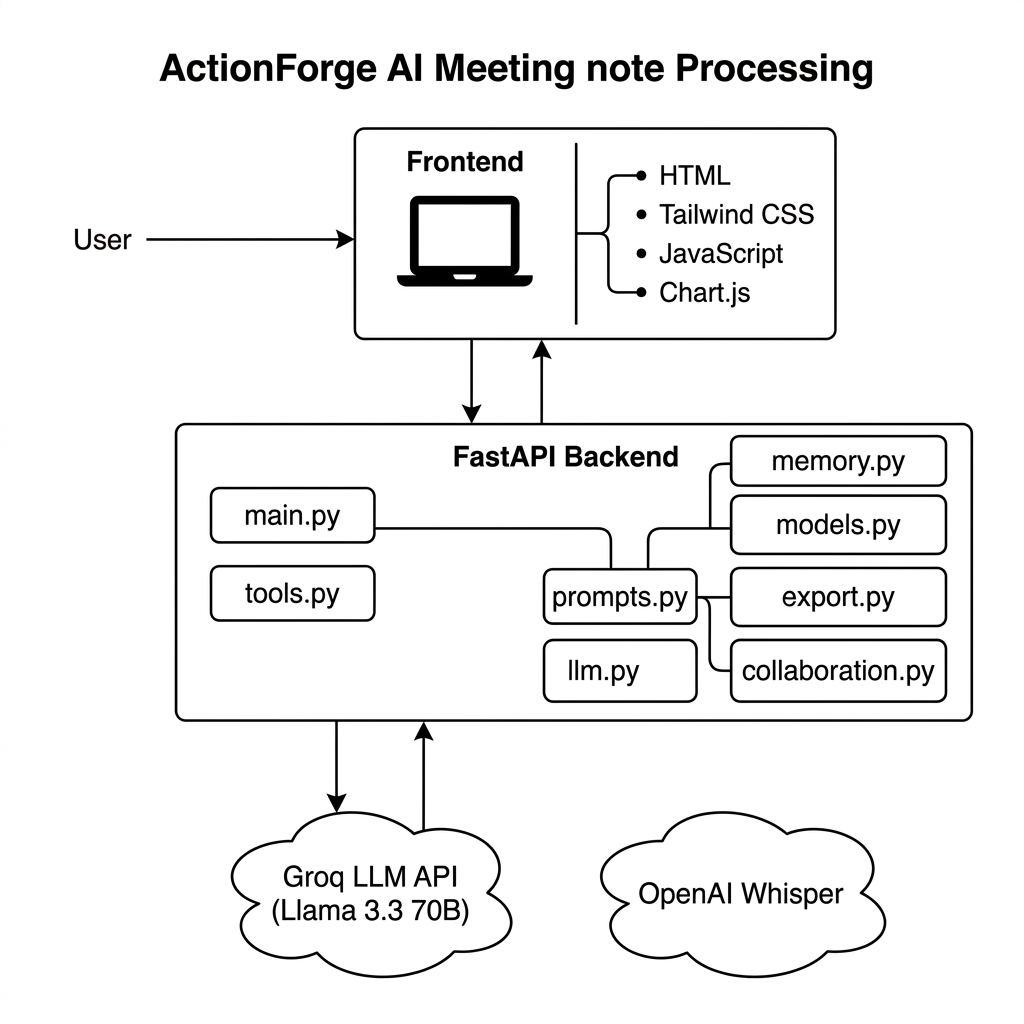
\includegraphics[width=\textwidth]{screenshots/img01_architecture.png}
\caption{System Architecture --- Frontend, FastAPI Backend, Groq LLM API, Session Memory flow}
\end{figure}

\subsection*{Frontend Layer}
The frontend acts as the user interaction layer where users paste meeting notes, select dates, upload audio, and view generated action plans. It is a single-page HTML application styled with Tailwind CSS (CDN) and uses vanilla JavaScript for API communication and Chart.js for analytics visualizations.

\subsection*{Backend Layer}
The backend is built using FastAPI and handles all core processing. It manages API requests, processes meeting notes through the 5-stage AI pipeline, maintains session memory, handles user authentication, manages collaboration sessions, and generates PDF/CSV exports.

\subsection*{AI Layer}
The system integrates the Groq API with Llama 3.3 70B (primary) and Llama 3.1 8B (fallback) for all AI-powered text processing. Structured Prompt Templates guide the LLM through each analysis stage.

\subsection*{External APIs / Services}
The system uses the Groq API for LLM-powered text analysis and OpenAI Whisper API for audio transcription. All API communication is handled securely through environment variables.

\subsection{High-Level Architecture Diagram}

\begin{figure}[H]
\centering
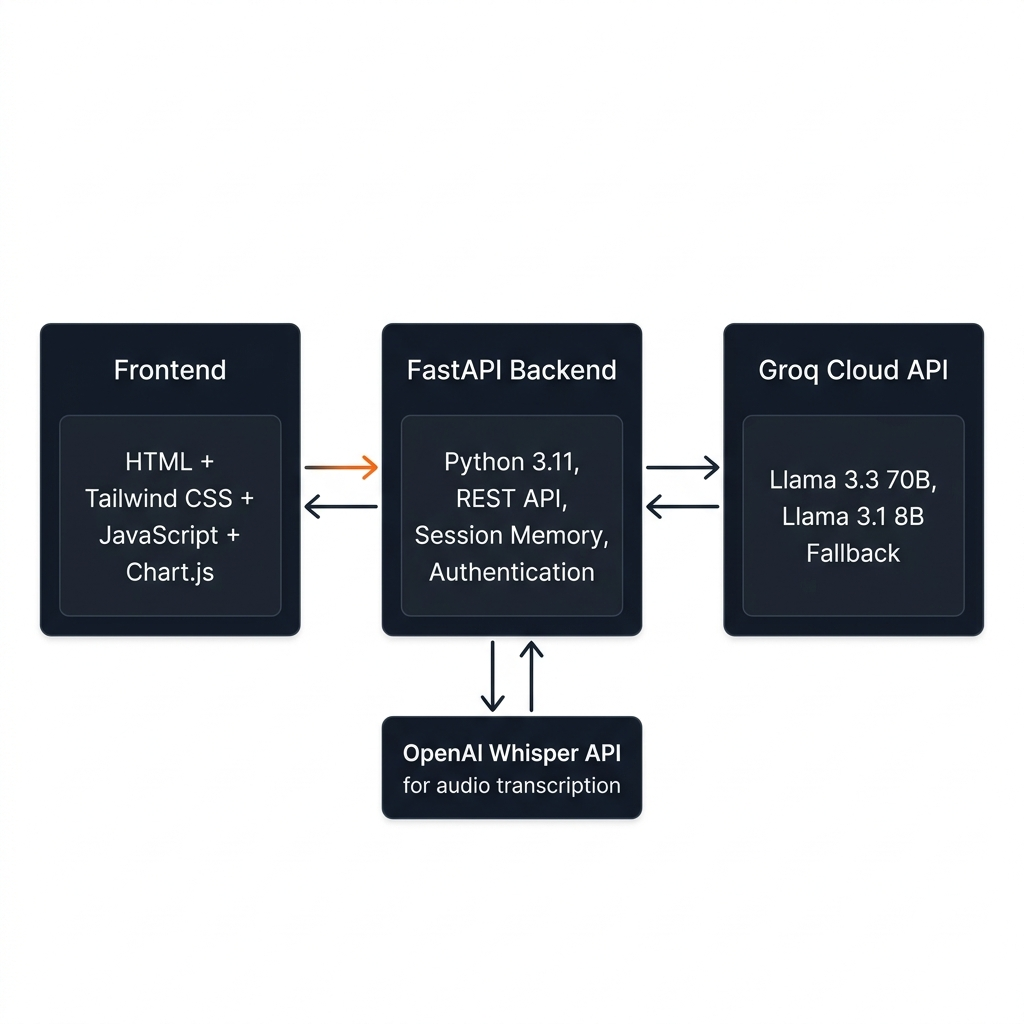
\includegraphics[width=\textwidth]{screenshots/img02_highlevel_arch.png}
\caption{High-Level Architecture Diagram}
\end{figure}

\subsection{Component Interaction Diagram}

\begin{figure}[H]
\centering
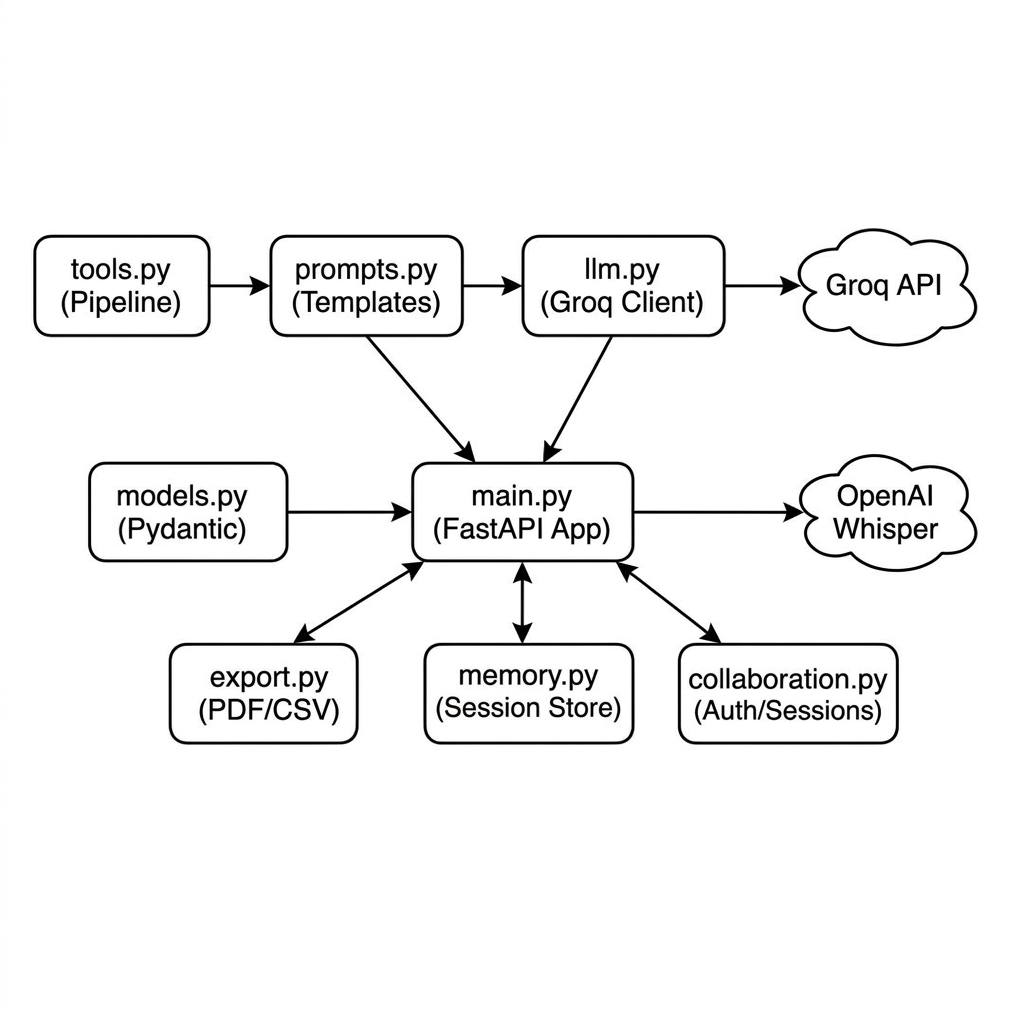
\includegraphics[width=\textwidth]{screenshots/img03_component_interaction.png}
\caption{Component Interaction Diagram}
\end{figure}


% ══════════════════════════════════════════════════════════════
\section{Pre-requisites}

\subsection{Software Requirements}
\begin{itemize}
  \item \textbf{Python:} Version 3.9 or higher (Python 3.11 recommended)
  \item \textbf{pip:} Python package manager for installing project dependencies
  \item \textbf{IDE:} Visual Studio Code with Python extension or any preferred code editor
  \item \textbf{Browser:} Modern web browser (Chrome, Edge, Firefox) supporting ES6, async/await, and Fetch API
  \item \textbf{Git:} Version control system for project management (optional but recommended)
\end{itemize}

\subsection{Libraries / Frameworks / Dependencies}
Install required dependencies using:
\begin{lstlisting}[language=bash]
pip install fastapi uvicorn groq pydantic python-dotenv reportlab python-multipart openai
\end{lstlisting}

\begin{itemize}
  \item \textbf{FastAPI (0.115.0):} Web framework for REST API routing and request handling
  \item \textbf{Uvicorn (0.30.6):} ASGI server for running the FastAPI application
  \item \textbf{Groq ($\geq$0.12.0):} Client library for accessing Groq LLM API
  \item \textbf{Pydantic (2.9.2):} Data validation and serialization models
  \item \textbf{python-dotenv (1.0.1):} Environment variable management from .env files
  \item \textbf{ReportLab (4.0.9):} PDF generation library for export functionality
  \item \textbf{python-multipart (0.0.6):} File upload handling for audio transcription
  \item \textbf{OpenAI ($\geq$1.0.0):} Client library for Whisper audio transcription API
\end{itemize}

\subsection{Hardware Requirements}
\begin{itemize}
  \item \textbf{CPU:} Minimum Intel Core i3 or AMD Ryzen 3 processor (AI processing is cloud-based via Groq)
  \item \textbf{RAM:} Minimum 4 GB (8 GB recommended for smooth development)
  \item \textbf{Storage:} At least 500 MB free disk space for project files and dependencies
  \item \textbf{Network:} Stable internet connection required for Groq API and OpenAI Whisper API calls
\end{itemize}


% ══════════════════════════════════════════════════════════════
\section{Prior Knowledge Required}

\subsection{Programming Language Knowledge}
\begin{itemize}
  \item Strong understanding of Python fundamentals (variables, loops, functions, modules)
  \item Knowledge of object-oriented programming (OOP) concepts
  \item Familiarity with handling JSON data and working with APIs
  \item Basic understanding of error handling and debugging techniques
\end{itemize}

\subsection{Framework Basics}
\begin{itemize}
  \item Understanding of FastAPI framework for building RESTful APIs
  \item Knowledge of API routing, request/response handling, and status codes
  \item Familiarity with asynchronous programming (async/await) in Python
  \item Basic understanding of middleware (CORS) and dependency injection in FastAPI
\end{itemize}

\subsection{AI / NLP Fundamentals}
\begin{itemize}
  \item Basic understanding of Large Language Models (LLMs) and their capabilities
  \item Knowledge of prompt engineering and structured prompt templates
  \item Familiarity with API-based AI services (Groq, OpenAI)
  \item Understanding of how text generation models process and produce outputs
  \item Awareness of prompt engineering basics for effective AI responses
\end{itemize}

\subsection{Frontend Basics}
\begin{itemize}
  \item Understanding of HTML, CSS, and JavaScript fundamentals
  \item Familiarity with Fetch API for making HTTP requests
  \item Basic knowledge of DOM manipulation and event handling
  \item Understanding of responsive design and CSS frameworks (Tailwind CSS)
\end{itemize}


% ══════════════════════════════════════════════════════════════
\section{Project Objectives (Detailed)}

\subsection{Technical Objectives}
\begin{itemize}
  \item Design and develop a scalable meeting intelligence system using Python and FastAPI
  \item Implement a 5-stage AI tool pipeline for sequential meeting note processing
  \item Build structured Prompt Templates for each analysis stage
  \item Integrate Groq LLM API with automatic model fallback (Llama 3.3 70B $\rightarrow$ Llama 3.1 8B)
  \item Develop a session memory system for cross-meeting context retention
  \item Create RESTful API endpoints for all core functionalities
\end{itemize}

\subsection{Performance Objectives}
\begin{itemize}
  \item Ensure fast API response times for real-time meeting note processing
  \item Maintain reliable LLM responses with dual-model fallback strategy
  \item Achieve accurate task extraction and deadline detection from unstructured text
  \item Provide reliable export generation (PDF/CSV) with minimal latency
  \item Optimize system for low latency in AI-generated outputs
\end{itemize}

\subsection{Deployment Objectives}
\begin{itemize}
  \item Enable local development with simple setup (single pip install, single uvicorn command)
  \item Ensure secure handling of API keys using environment variables (.env files)
  \item Support cross-platform access via web browser
  \item Design for cloud deployment readiness
  \item Maintain high availability and reliability of backend services
\end{itemize}

\subsection{Learning Outcomes}
\begin{itemize}
  \item Gain hands-on experience in building real-world AI-powered applications
  \item Understand integration of LLM APIs with structured prompt engineering
  \item Learn FastAPI development with Pydantic models
  \item Develop skills in API design, system architecture, and data flow management
  \item Improve knowledge of AI-driven text processing and NLP approaches
\end{itemize}


% ══════════════════════════════════════════════════════════════
\section{Project Workflow}

% ──────────────────────────────────────────────────
\subsection{Milestone 1: Requirement Analysis \& System Design}

\subsubsection{Activity 1.1: Problem Definition}
Identify the need for an intelligent meeting note processing system that not only records discussions but also extracts actionable outputs. Address the limitation of traditional note-taking tools that lack automatic task extraction, deadline detection, and follow-up generation. Design a solution that integrates text processing, AI-powered analysis, and structured output generation to help sales teams improve accountability, follow-through, and communication efficiency. Ensure the system is scalable, user-friendly, and capable of transforming raw meeting text into comprehensive action plans using LLM APIs and Prompt Templates.

\subsubsection{Activity 1.2: Functional Requirements}
\begin{itemize}
  \item \textbf{FR-01:} Accept unstructured meeting notes as text input through a web interface
  \item \textbf{FR-02:} Support optional meeting date input for accurate deadline calculation
  \item \textbf{FR-03:} Generate executive summaries capturing key discussion points and decisions
  \item \textbf{FR-04:} Extract individual action items with priority classification (High/Medium/Low)
  \item \textbf{FR-05:} Detect deadlines from contextual clues and classify urgency (Immediate/Soon/Flexible)
  \item \textbf{FR-06:} Identify and assign roles/responsibilities to team members mentioned in notes
  \item \textbf{FR-07:} Draft professional follow-up emails with all extracted information
  \item \textbf{FR-08:} Maintain session memory for cross-meeting context continuity
  \item \textbf{FR-09:} Export action plans as PDF and CSV documents
  \item \textbf{FR-10:} Transcribe audio meeting recordings to text using Whisper API
  \item \textbf{FR-11:} Expose RESTful API endpoints for all functionalities
\end{itemize}

\subsubsection{Activity 1.3: Non-Functional Requirements}
\begin{itemize}
  \item \textbf{NFR-01 Performance:} API responses should complete within 10 seconds for full pipeline
  \item \textbf{NFR-02 Reliability:} Dual-model fallback ensures operation even if primary model fails
  \item \textbf{NFR-03 Scalability:} Modular architecture supports future feature additions
  \item \textbf{NFR-04 Security:} API keys managed through .env files, CORS configured
  \item \textbf{NFR-05 Maintainability:} Separation of concerns with distinct modules
  \item \textbf{NFR-06 Usability:} Clean, modern UI with intuitive input/output flow
\end{itemize}

\subsubsection{Activity 1.4: System Design \& Technology Selection}
\begin{itemize}
  \item \textbf{Backend Framework:} Use FastAPI for high-performance API development and async request handling
  \item \textbf{AI Integration:} Use Groq-powered LLMs (Llama 3.3 70B) for text analysis, summarization, and content generation
  \item \textbf{Prompt Engineering:} Design structured Prompt Templates for each of the 5 pipeline stages
  \item \textbf{Session Memory:} Implement in-memory context store for cross-meeting continuity
  \item \textbf{Frontend:} Single-page HTML with Tailwind CSS (CDN) and vanilla JavaScript
  \item \textbf{Export:} ReportLab for PDF, Python csv for CSV exports
  \item \textbf{Audio:} OpenAI Whisper API for speech-to-text transcription
  \item \textbf{Environment Configuration:} Use .env files to securely manage API keys
\end{itemize}

% ──────────────────────────────────────────────────
\subsection{Milestone 2: Environment Setup \& Initial Configuration}

\subsubsection{Activity 2.1: Development Environment Setup}
\begin{itemize}
  \item Install Python 3.11 from the official Python website and ensure ``Add Python to PATH'' is enabled during installation
  \item Install Visual Studio Code with the Python extension for development
  \item Create the main project directory: \texttt{mkdir actionforge \&\& cd actionforge}
  \item Create backend and frontend directories: \texttt{mkdir backend frontend}
  \item Create and activate a virtual environment: \texttt{python -m venv venv}
  \item Activate: \texttt{venv\textbackslash Scripts\textbackslash activate} (Windows) or \texttt{source venv/bin/activate} (Linux/Mac)
\end{itemize}

\begin{figure}[H]
\centering
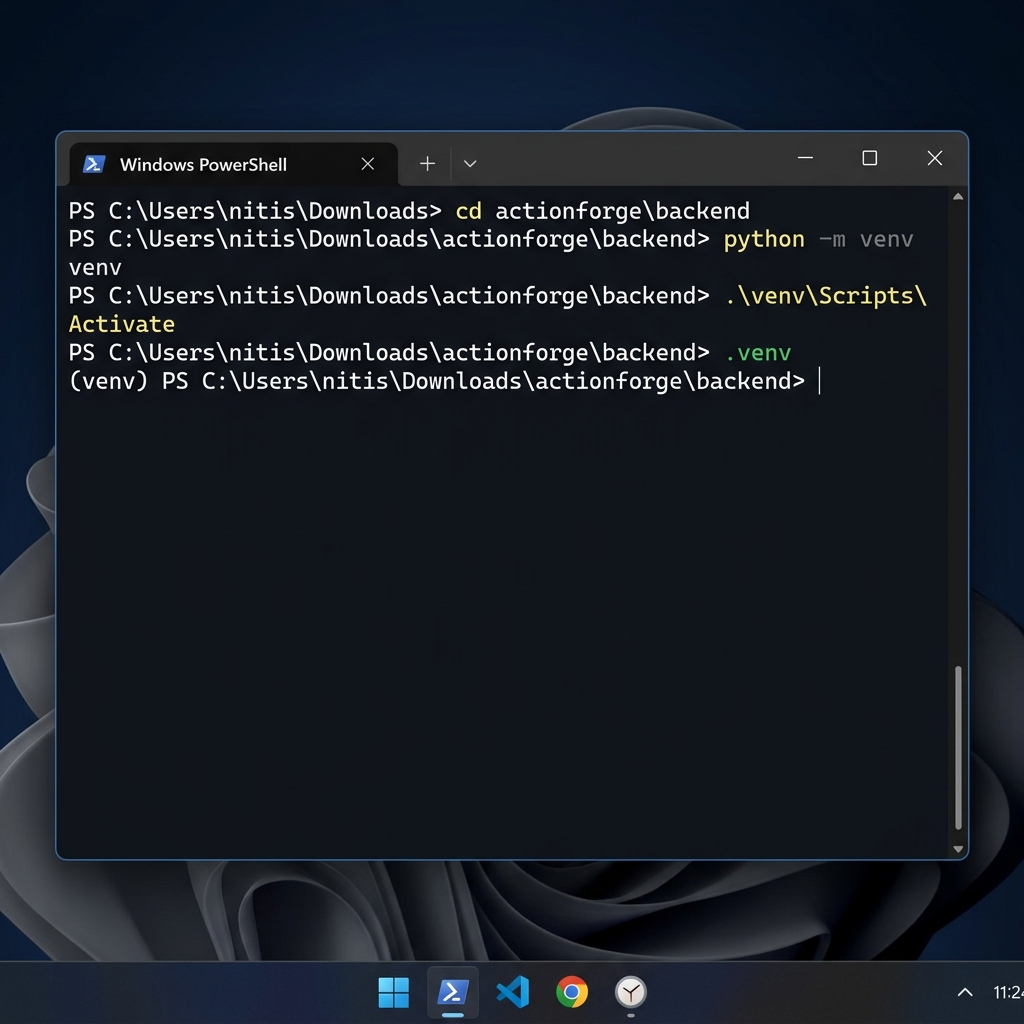
\includegraphics[width=0.8\textwidth]{screenshots/img04_terminal_venv.png}
\caption{Virtual environment activated in terminal}
\end{figure}

\subsubsection{Activity 2.2: Dependency Installation}
Install all required Python libraries using pip:
\begin{lstlisting}[language=bash]
pip install -r requirements.txt
\end{lstlisting}

\texttt{requirements.txt} contents:
\begin{lstlisting}
fastapi==0.115.0
uvicorn==0.30.6
groq>=0.12.0
pydantic==2.9.2
python-dotenv==1.0.1
reportlab==4.0.9
python-multipart==0.0.6
openai>=1.0.0
\end{lstlisting}

\subsubsection{Activity 2.3: Project Structure Creation}
Organize the project into a clean and modular folder structure by separating LLM logic, tools, prompts, models, memory, and export functions into individual files. This ensures better code readability, maintainability, and scalability while enabling smooth integration of different components.

\begin{figure}[H]
\centering
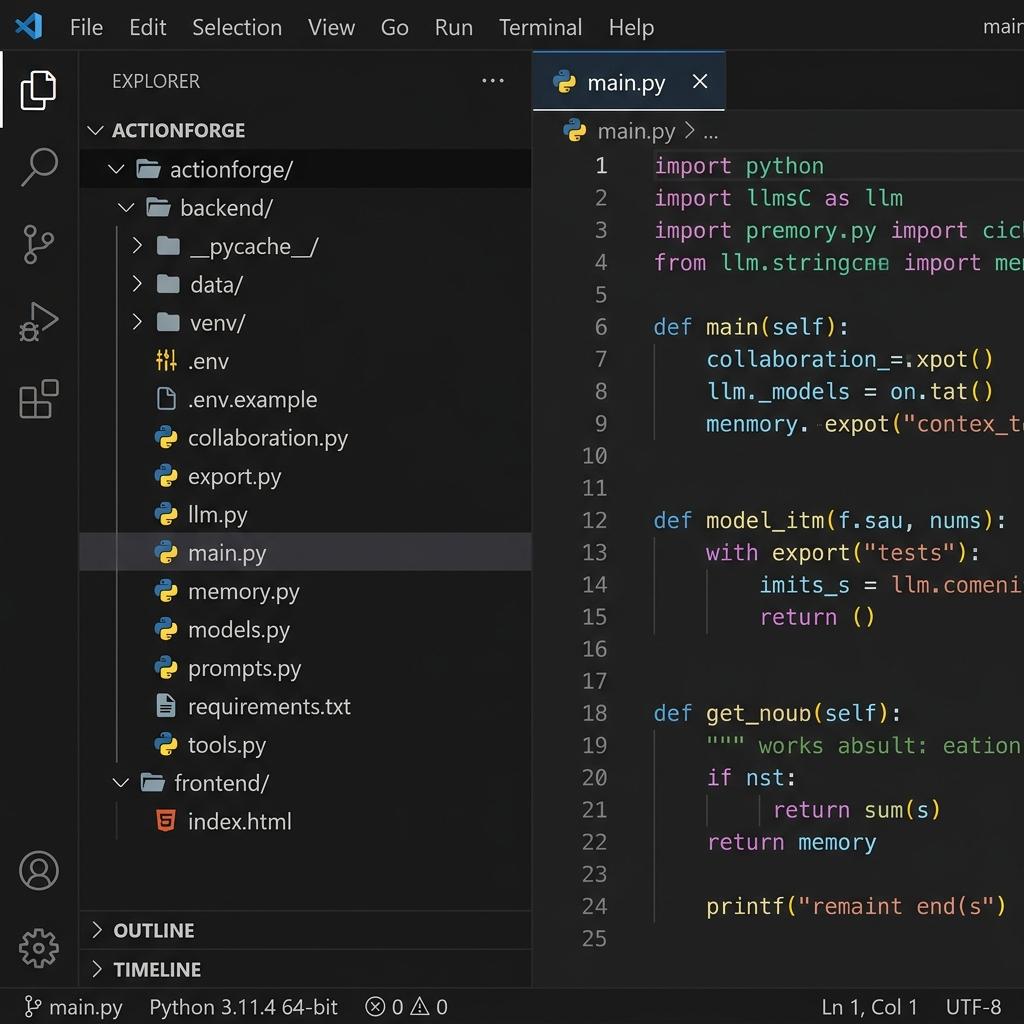
\includegraphics[width=0.4\textwidth]{screenshots/img05_folder_structure.png}
\caption{Project Folder Structure in VS Code}
\end{figure}

\subsubsection{Activity 2.4: Configuration Setup}
Set up the application configuration by defining environment variables required for secure and efficient operation. This includes storing API keys (Groq, OpenAI) in a \texttt{.env} file. Configure the LLM client initialization, model selection, and ensure all services are properly integrated.


% ──────────────────────────────────────────────────
\subsection{Milestone 3: API Key Setup}

\subsubsection{Activity 3.1: Create Groq Account \& Get API Key}

\textbf{Step 1: Create Groq Account}
\begin{enumerate}
  \item Go to Groq Console: \url{https://console.groq.com}
  \item Click ``Sign Up'' or ``Get Started''
  \item Sign up with GitHub or Google (Free, no credit card required)
  \item Verify your email if needed
\end{enumerate}

\begin{figure}[H]
\centering
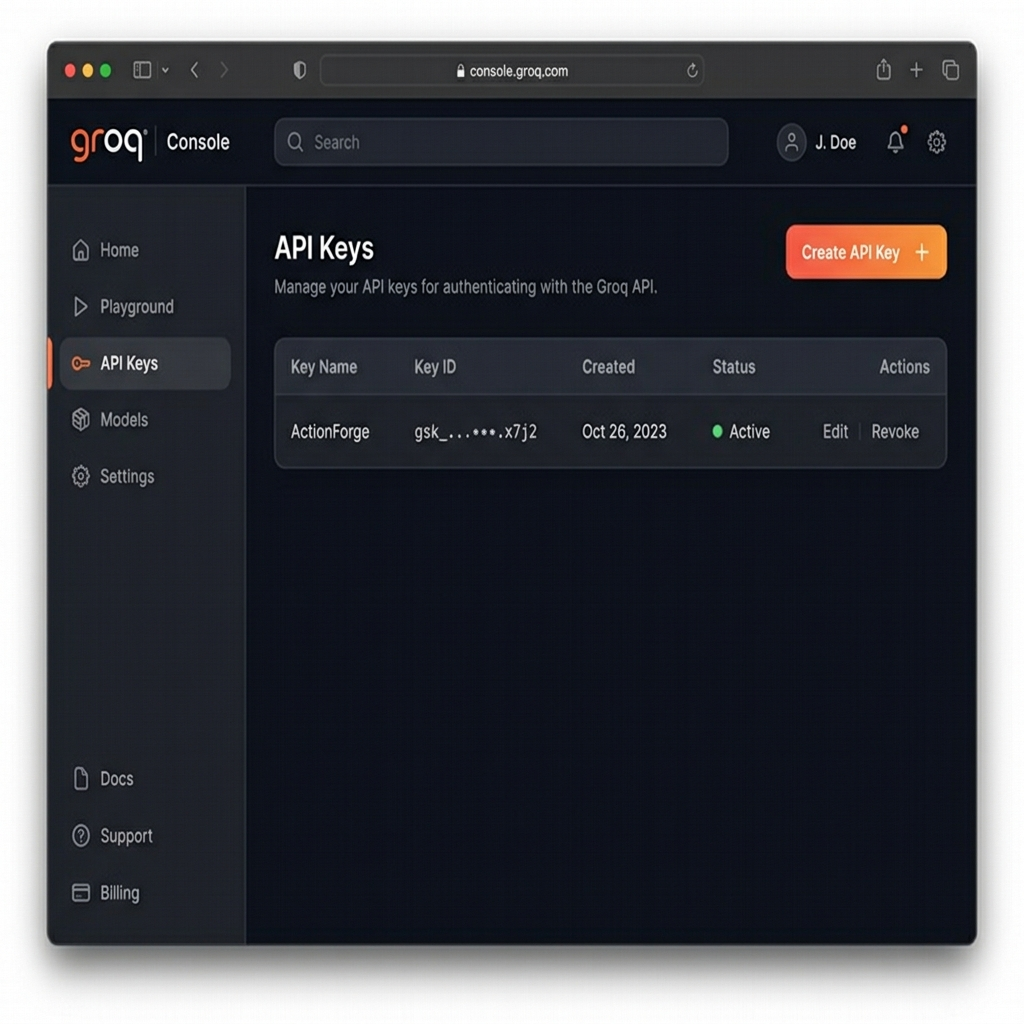
\includegraphics[width=0.8\textwidth]{screenshots/img06_groq_console.png}
\caption{Groq Console Dashboard}
\end{figure}

\begin{figure}[H]
\centering
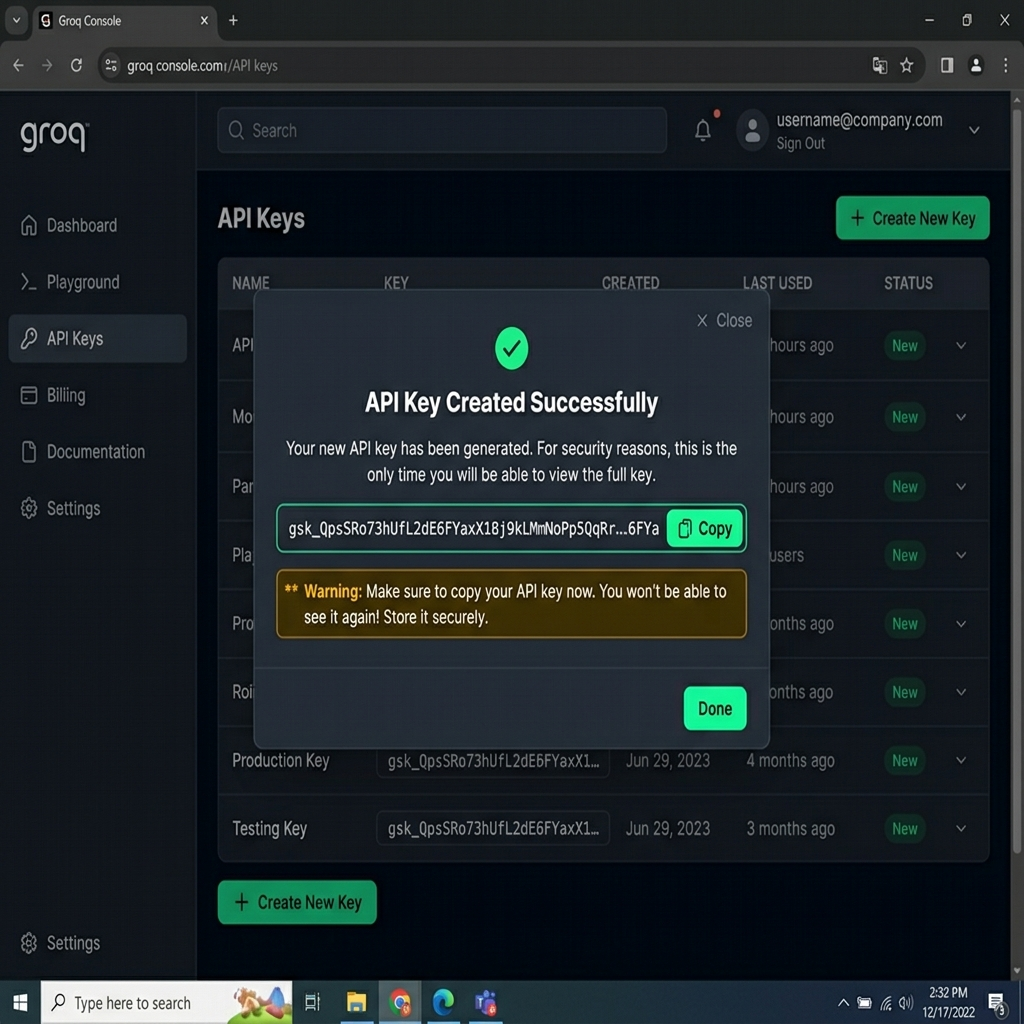
\includegraphics[width=0.8\textwidth]{screenshots/img09_groq_key_created.png}
\caption{New API Key Created}
\end{figure}


\subsubsection{Activity 3.2: Create .env Configuration File}

\begin{enumerate}
  \item Navigate to the \texttt{backend/} directory
  \item Create a new file named \texttt{.env} (not \texttt{.env.txt})
\end{enumerate}

\begin{figure}[H]
\centering
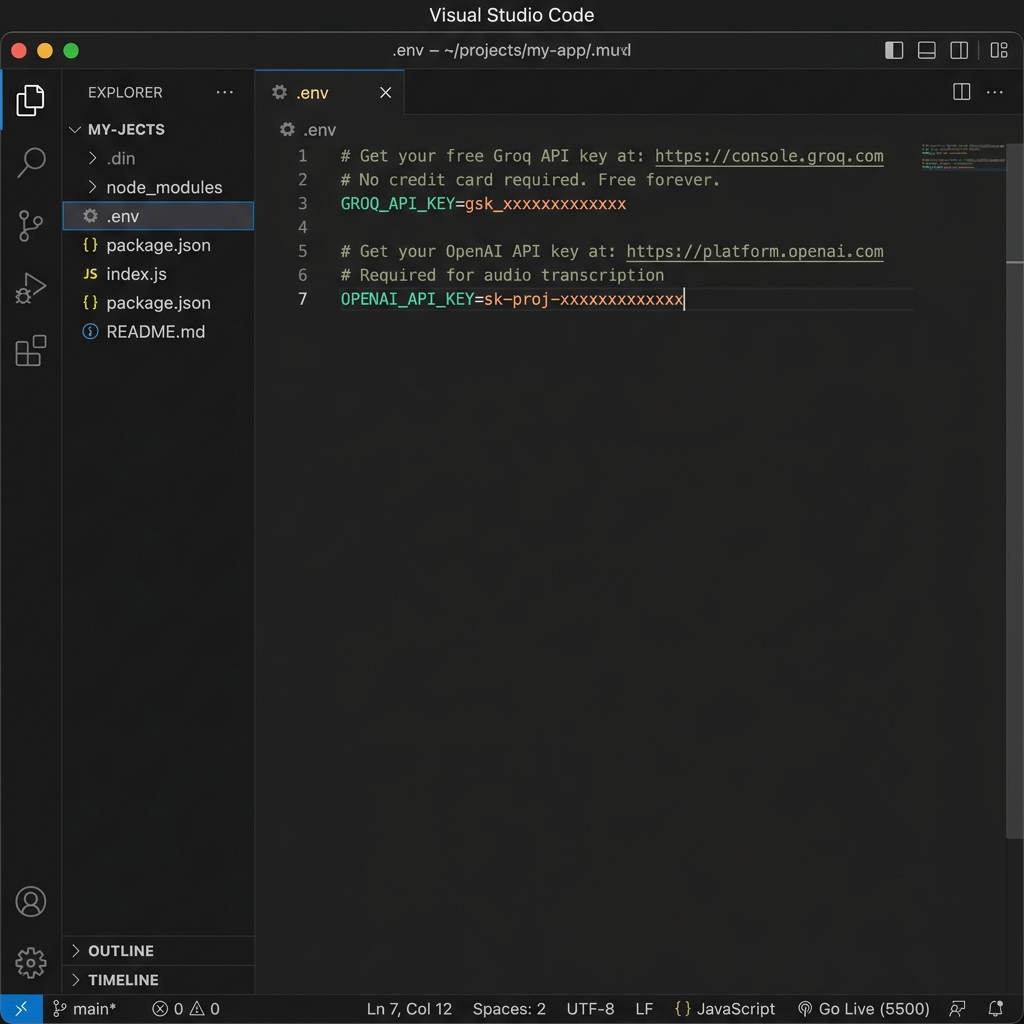
\includegraphics[width=0.8\textwidth]{screenshots/img12_env_file.png}
\caption{	exttt{.env} File Configuration}
\end{figure}


% ──────────────────────────────────────────────────
\subsection{Milestone 4: Core System Development}

\subsubsection{Activity 4.1: Prompt Templates Module (\texttt{prompts.py})}
This module defines structured system and user prompts for each of the 5 pipeline stages. Each prompt template is carefully engineered to guide the LLM to produce consistent, formatted outputs. The prompts define the AI's persona, expected output format, and context handling for summary generation, task extraction, deadline detection, role assignment, and email drafting.

\begin{figure}[H]
\centering
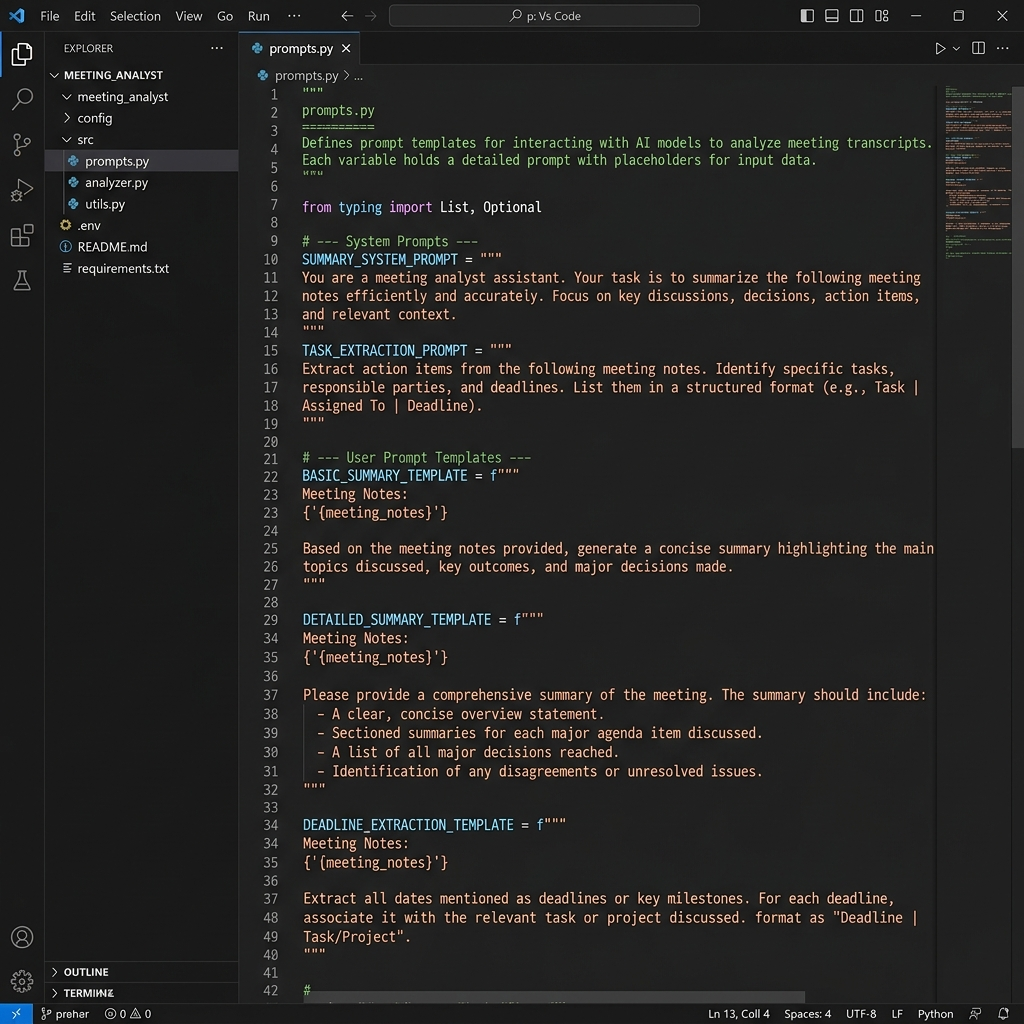
\includegraphics[width=\textwidth]{screenshots/img14_prompts_code.png}
\caption{	exttt{prompts.py} Code snippet}
\end{figure}

\subsubsection{Activity 4.2: Tool Pipeline Module (\texttt{tools.py})}
This component implements the five MCP-style tool functions that combine prompt templates with LLM calls. Each tool function takes meeting notes and optional context, constructs the appropriate prompt, calls the LLM, and returns the structured output. The tools are: \texttt{generate\_summary()}, \texttt{extract\_tasks()}, \texttt{extract\_deadlines()}, \texttt{assign\_roles()}, and \texttt{generate\_email()}.

\begin{figure}[H]
\centering
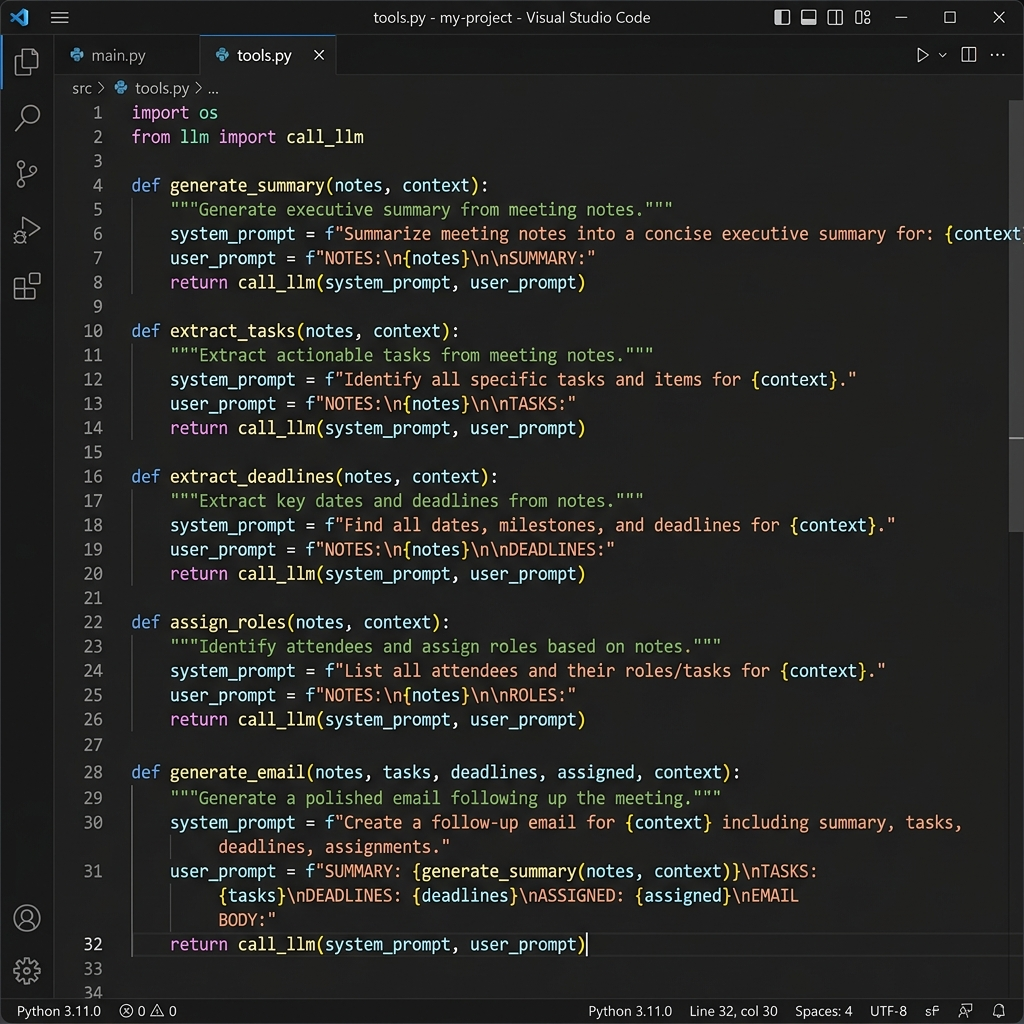
\includegraphics[width=\textwidth]{screenshots/img15_tools_code.png}
\caption{	exttt{tools.py} Code snippet}
\end{figure}

\subsubsection{Activity 4.3: LLM Integration Module (\texttt{llm.py})}
This module initializes the Groq client and provides the core \texttt{call\_llm()} function with dual-model fallback. It tries the primary model (Llama 3.3 70B) first, and automatically falls back to the secondary model (Llama 3.1 8B) if the primary fails. This ensures high availability of AI processing.

\begin{figure}[H]
\centering
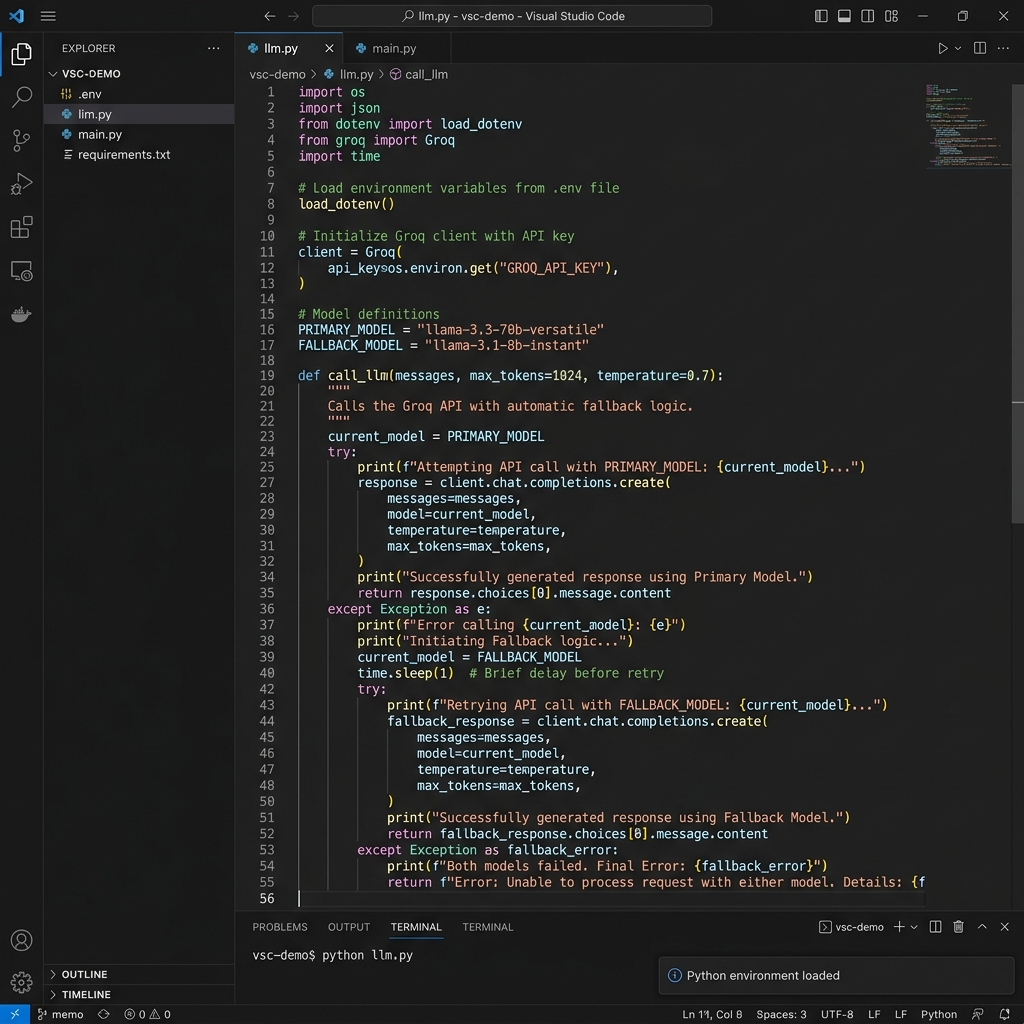
\includegraphics[width=\textwidth]{screenshots/img16_llm_code.png}
\caption{	exttt{llm.py} Full Code snippet}
\end{figure}

\subsubsection{Activity 4.4: FastAPI Application (\texttt{main.py})}
This is the main application file that defines all API endpoints using FastAPI. It includes the \texttt{/process\_notes} endpoint (main pipeline), \texttt{/memory} endpoints, \texttt{/transcribe\_audio}, \texttt{/export/pdf}, \texttt{/export/csv}, authentication endpoints (\texttt{/auth/register}, \texttt{/auth/login}), and collaboration session endpoints. CORS middleware is configured for cross-origin access.

\begin{figure}[H]
\centering
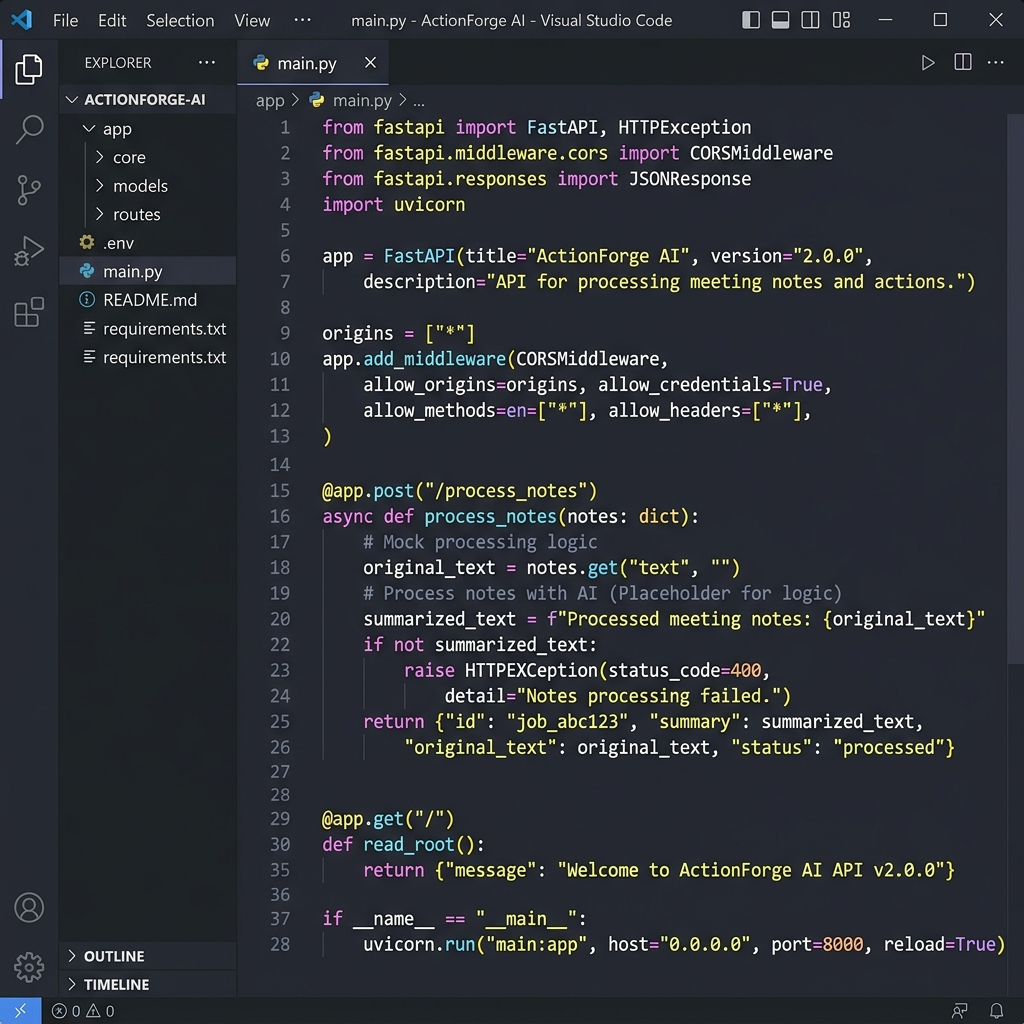
\includegraphics[width=\textwidth]{screenshots/img17_mainpy_code.png}
\caption{	exttt{main.py} Initialization Code}
\end{figure}


% ──────────────────────────────────────────────────
\subsection{Milestone 5: Integration \& Optimization}

\subsubsection{Activity 5.1: Component Integration (Frontend, Backend, AI)}
This activity focuses on connecting all system components. The frontend JavaScript fetch calls are mapped to FastAPI backend endpoints at \texttt{http://localhost:8000}. The backend is connected to the Groq LLM API for AI processing. Proper API mapping, data flow validation, and synchronization between components are ensured.

\subsubsection{Activity 5.2: Performance Optimization}
API response times are improved through efficient prompt engineering, minimal token usage, and optimized data processing. The dual-model fallback reduces downtime. Async request handling in FastAPI ensures smooth concurrent operations.

\subsubsection{Activity 5.3: Security Enhancements}
Security measures include environment variable management for API keys, CORS middleware configuration, input validation using Pydantic models, and proper error handling to prevent information leakage.

\subsubsection{Activity 5.4: Error Handling \& Validation}
Comprehensive try/catch blocks with structured error responses. Pydantic models validate all incoming data. Frontend toast notifications display user-friendly error messages. Backend returns proper HTTP status codes.


% ──────────────────────────────────────────────────
\subsection{Milestone 6: Deployment}

\begin{figure}[H]
\centering
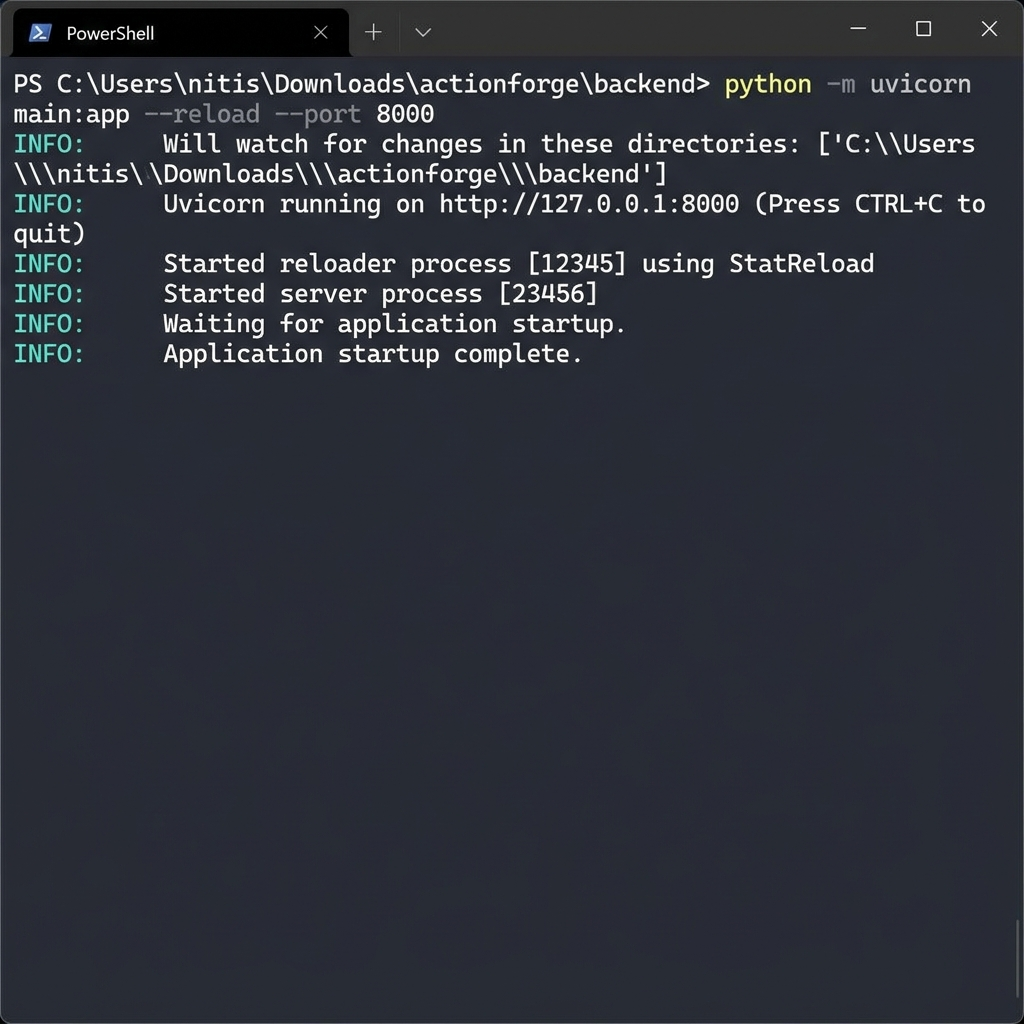
\includegraphics[width=0.8\textwidth]{screenshots/img18_server_start.png}
\caption{Starting Backend Server}
\end{figure}

\textbf{Backend Deployment Configuration:}
\begin{itemize}
  \item \textbf{Runtime:} Python 3.11
  \item \textbf{Framework:} FastAPI with Uvicorn ASGI server
  \item \textbf{Install Command:} \texttt{pip install -r requirements.txt}
  \item \textbf{Start Command:} \texttt{uvicorn main:app --host 0.0.0.0 --port 8000}
\end{itemize}

\begin{figure}[H]
\centering
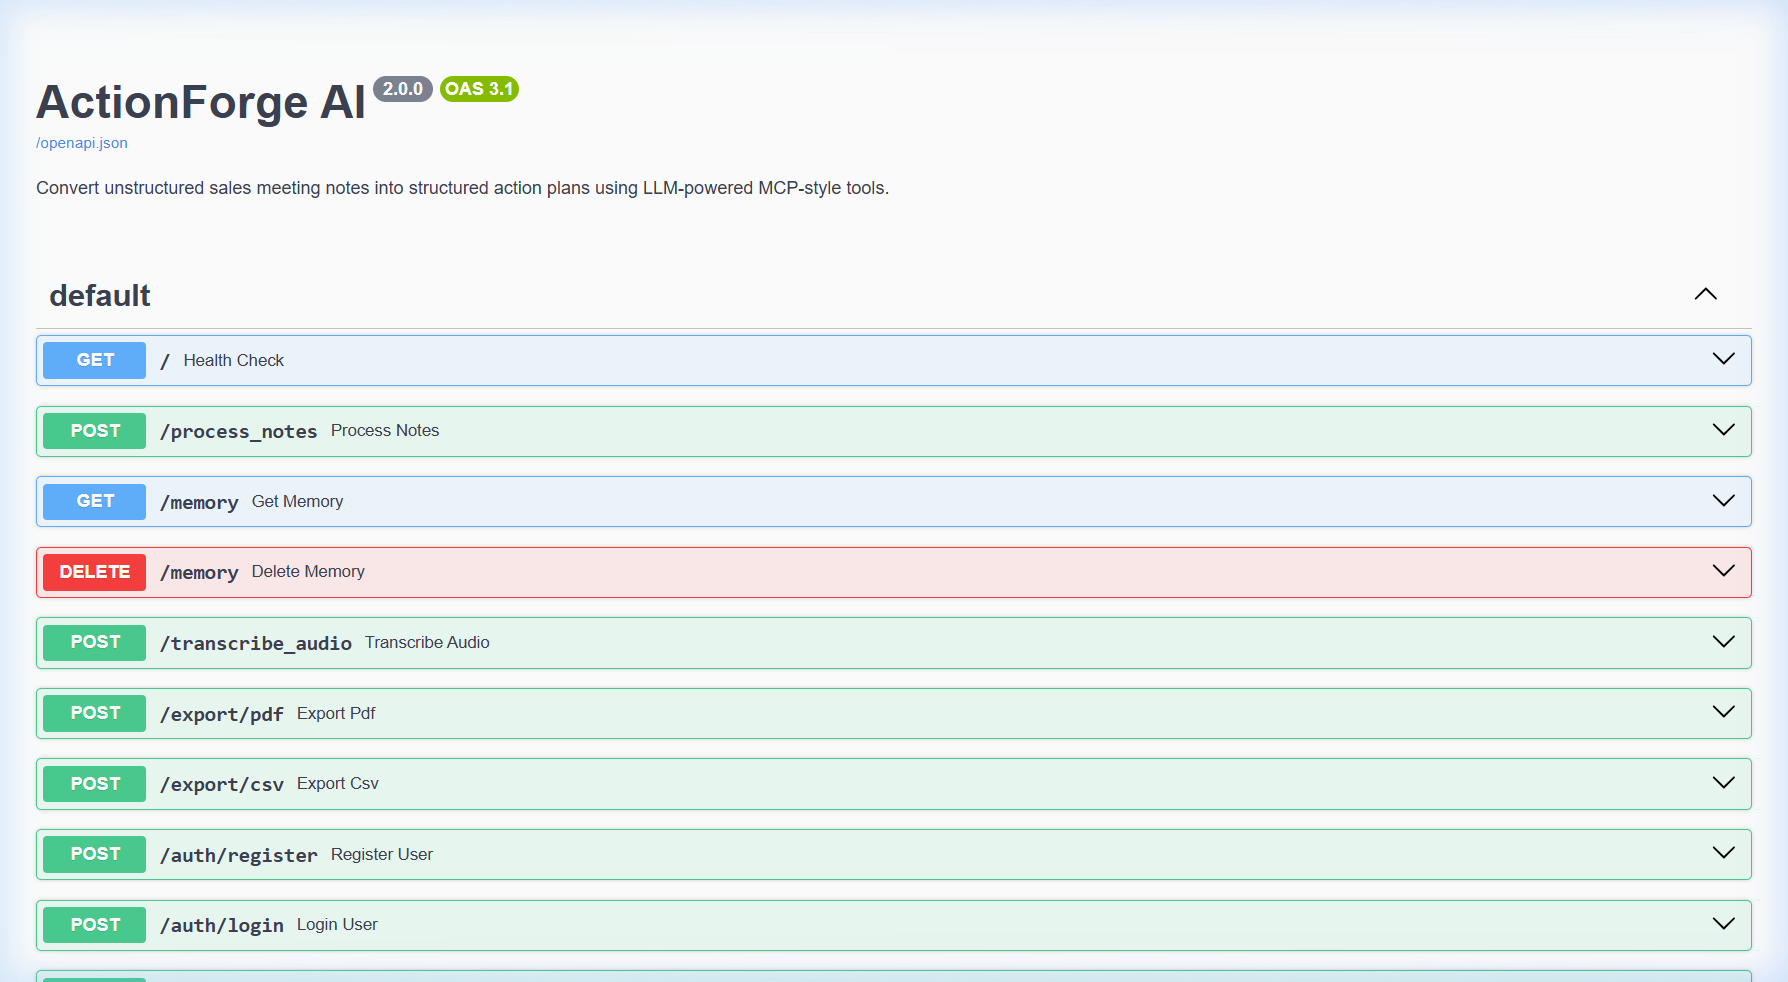
\includegraphics[width=\textwidth]{screenshots/img20_swagger_ui.png}
\caption{FastAPI Swagger UI Auto-generated Docs}
\end{figure}

\textbf{Environment Variables for Deployment:}
\begin{lstlisting}
GROQ_API_KEY=your_groq_api_key_here
OPENAI_API_KEY=your_openai_api_key_here
\end{lstlisting}

\begin{figure}[H]
\centering
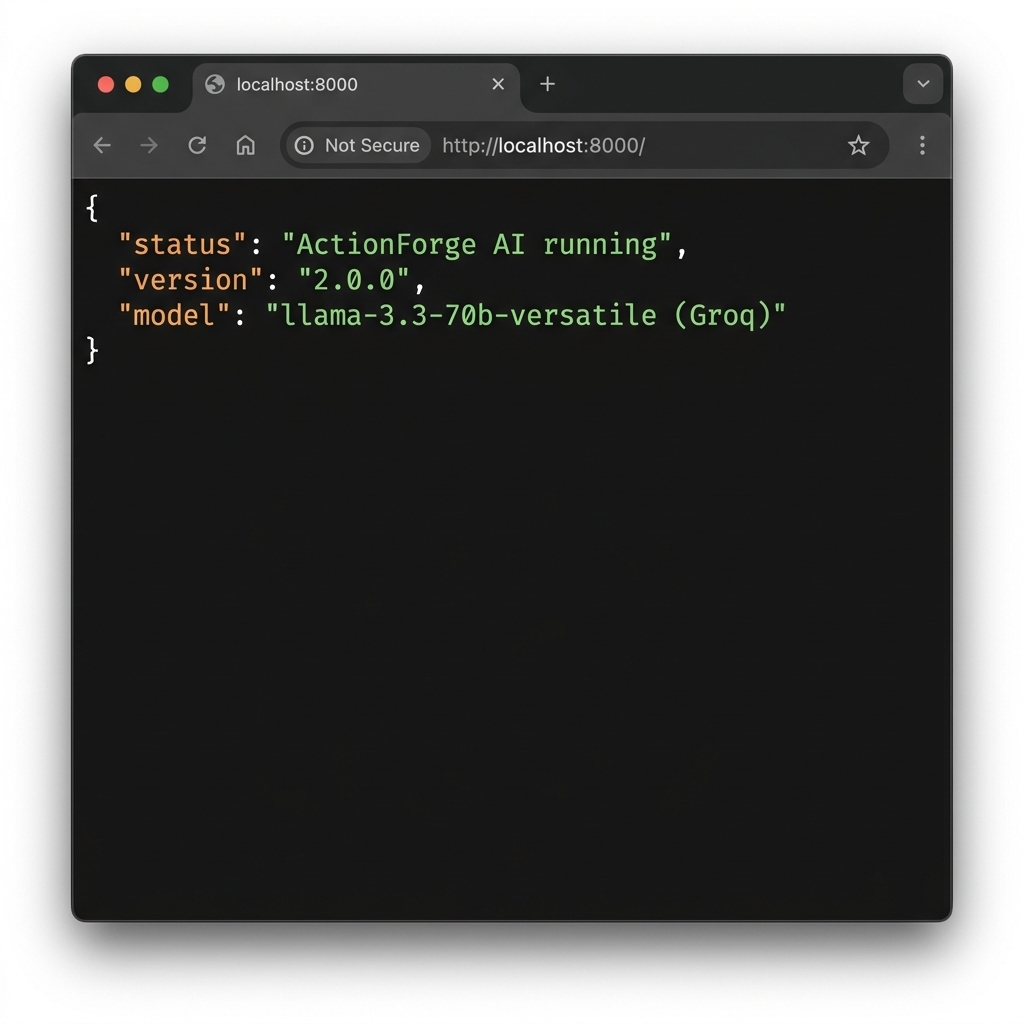
\includegraphics[width=0.8\textwidth]{screenshots/img23_health_check.png}
\caption{Health Check API Response}
\end{figure}


% ──────────────────────────────────────────────────
\subsection{Milestone 7: Testing \& Validation}

\subsubsection{Activity 7.1: Functional Test Case Execution}
Tested all core functionalities including note processing, memory management, audio transcription, PDF/CSV export, and authentication endpoints.

\begin{figure}[H]
\centering
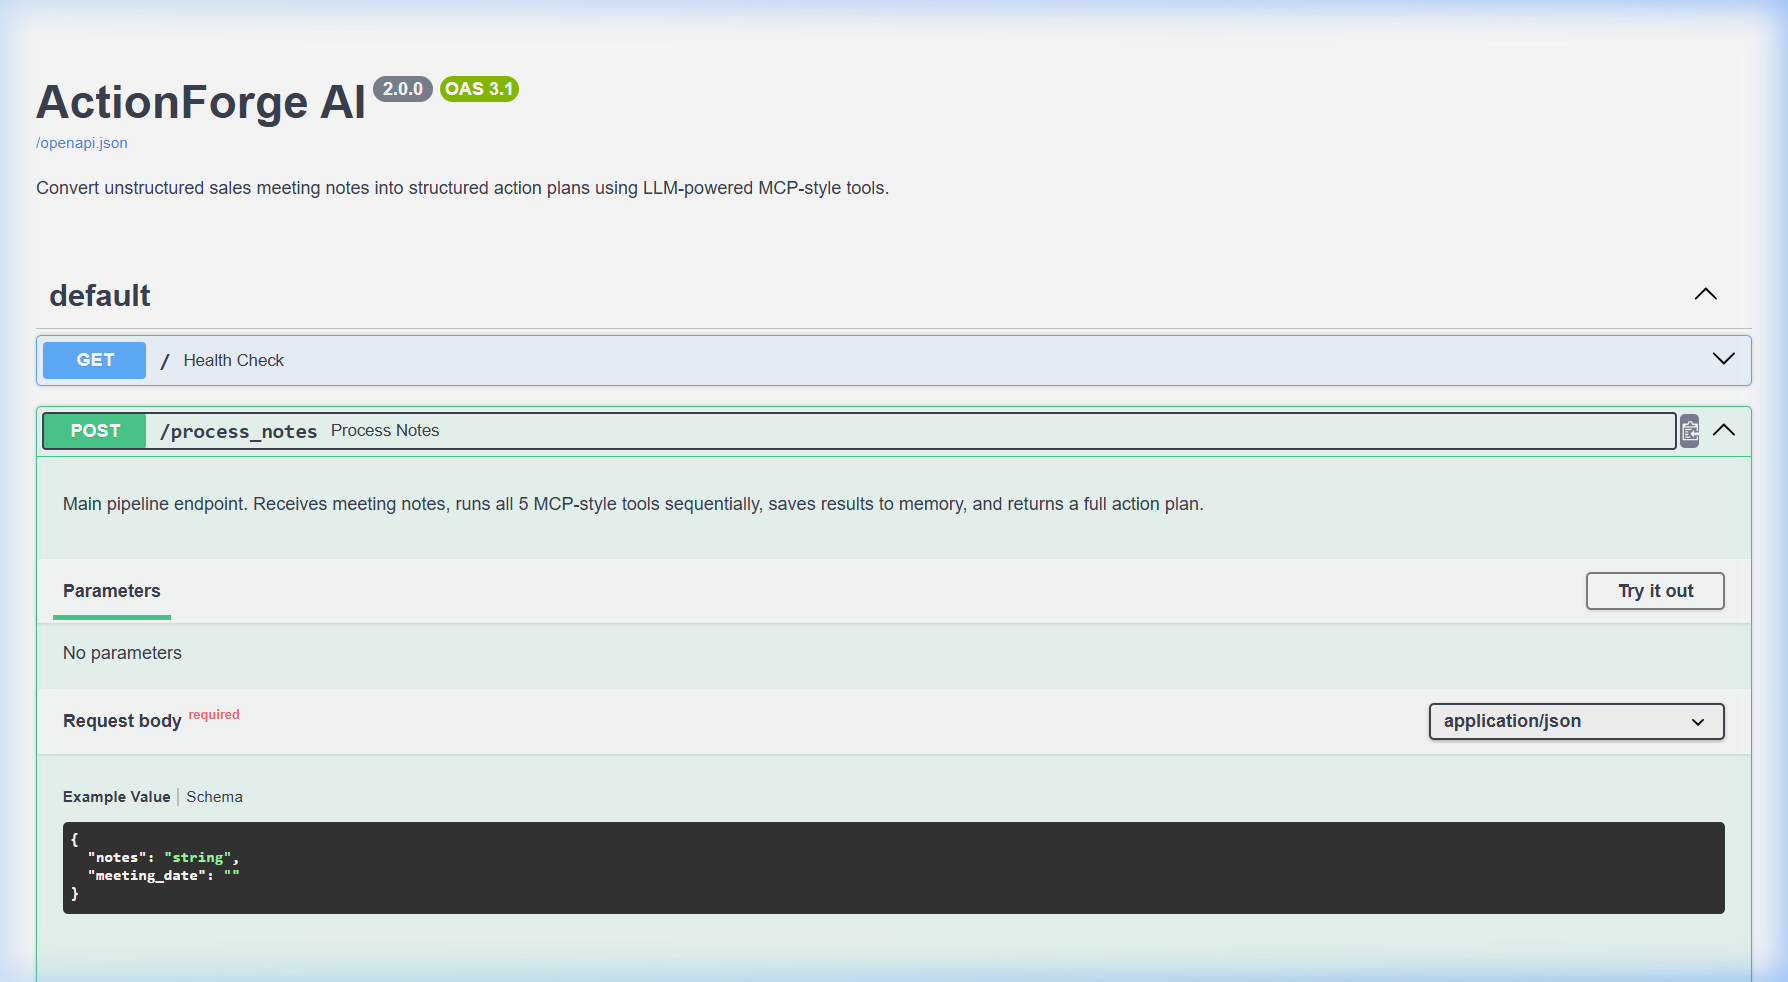
\includegraphics[width=0.8\textwidth]{screenshots/img27_swagger_process_notes.png}
\caption{Testing API Endpoints with Swagger}
\end{figure}


% ══════════════════════════════════════════════════════════════
\section{Project Directory Structure (Detailed)}

\begin{longtable}{|p{4.5cm}|p{9.5cm}|}
\hline
\textbf{File / Directory} & \textbf{Purpose} \\
\hline
\texttt{backend/} & Contains all backend Python source code and configuration \\
\hline
\texttt{backend/main.py} & FastAPI application entry point with all API endpoints, CORS middleware, request handlers for processing, export, authentication, and collaboration \\
\hline
\texttt{backend/llm.py} & Groq API client initialization and \texttt{call\_llm()} function with dual-model fallback strategy \\
\hline
\texttt{backend/prompts.py} & Structured prompt templates for each pipeline stage (summary, tasks, deadlines, roles, email) \\
\hline
\texttt{backend/tools.py} & Five MCP-style tool functions combining prompts with LLM calls \\
\hline
\texttt{backend/models.py} & Pydantic data models for request/response validation \\
\hline
\texttt{backend/memory.py} & In-memory session storage for cross-meeting context retention \\
\hline
\texttt{backend/export.py} & PDF generation (ReportLab) and CSV export functions \\
\hline
\texttt{backend/collaboration.py} & User management, authentication, shared sessions, permission system \\
\hline
\texttt{backend/requirements.txt} & Python dependency list for pip installation \\
\hline
\texttt{backend/.env} & Environment variables (Groq API key, OpenAI API key) --- not committed to Git \\
\hline
\texttt{backend/.env.example} & Template .env file with placeholder values for new developers \\
\hline
\texttt{frontend/} & Contains the frontend application \\
\hline
\texttt{frontend/index.html} & Complete single-page frontend (HTML + Tailwind CSS + JavaScript + Chart.js) \\
\hline
\end{longtable}


% ══════════════════════════════════════════════════════════════
\section{Results}

\subsection*{System Output}
The system successfully accepts raw meeting notes as text input and generates a comprehensive action plan through its 5-stage AI pipeline. It produces executive summaries, extracts prioritized tasks, detects deadlines with urgency classification, assigns roles, and drafts professional follow-up emails --- all within seconds.

\subsection*{Performance Evaluation}
The application demonstrates efficient performance with fast API response times (typically 5--10 seconds for full pipeline processing). The dual-model fallback ensures reliability. The frontend provides smooth, responsive interactions with animated pipeline progress indicators.

\subsection*{Screenshots}
The system includes user interface screens such as meeting input forms, pipeline animations, tabbed result views, analytics dashboards, and AI-generated outputs. These visuals demonstrate the working flow from data input to intelligent output generation.

\textbf{Landing Page:}

\begin{figure}[H]
\centering
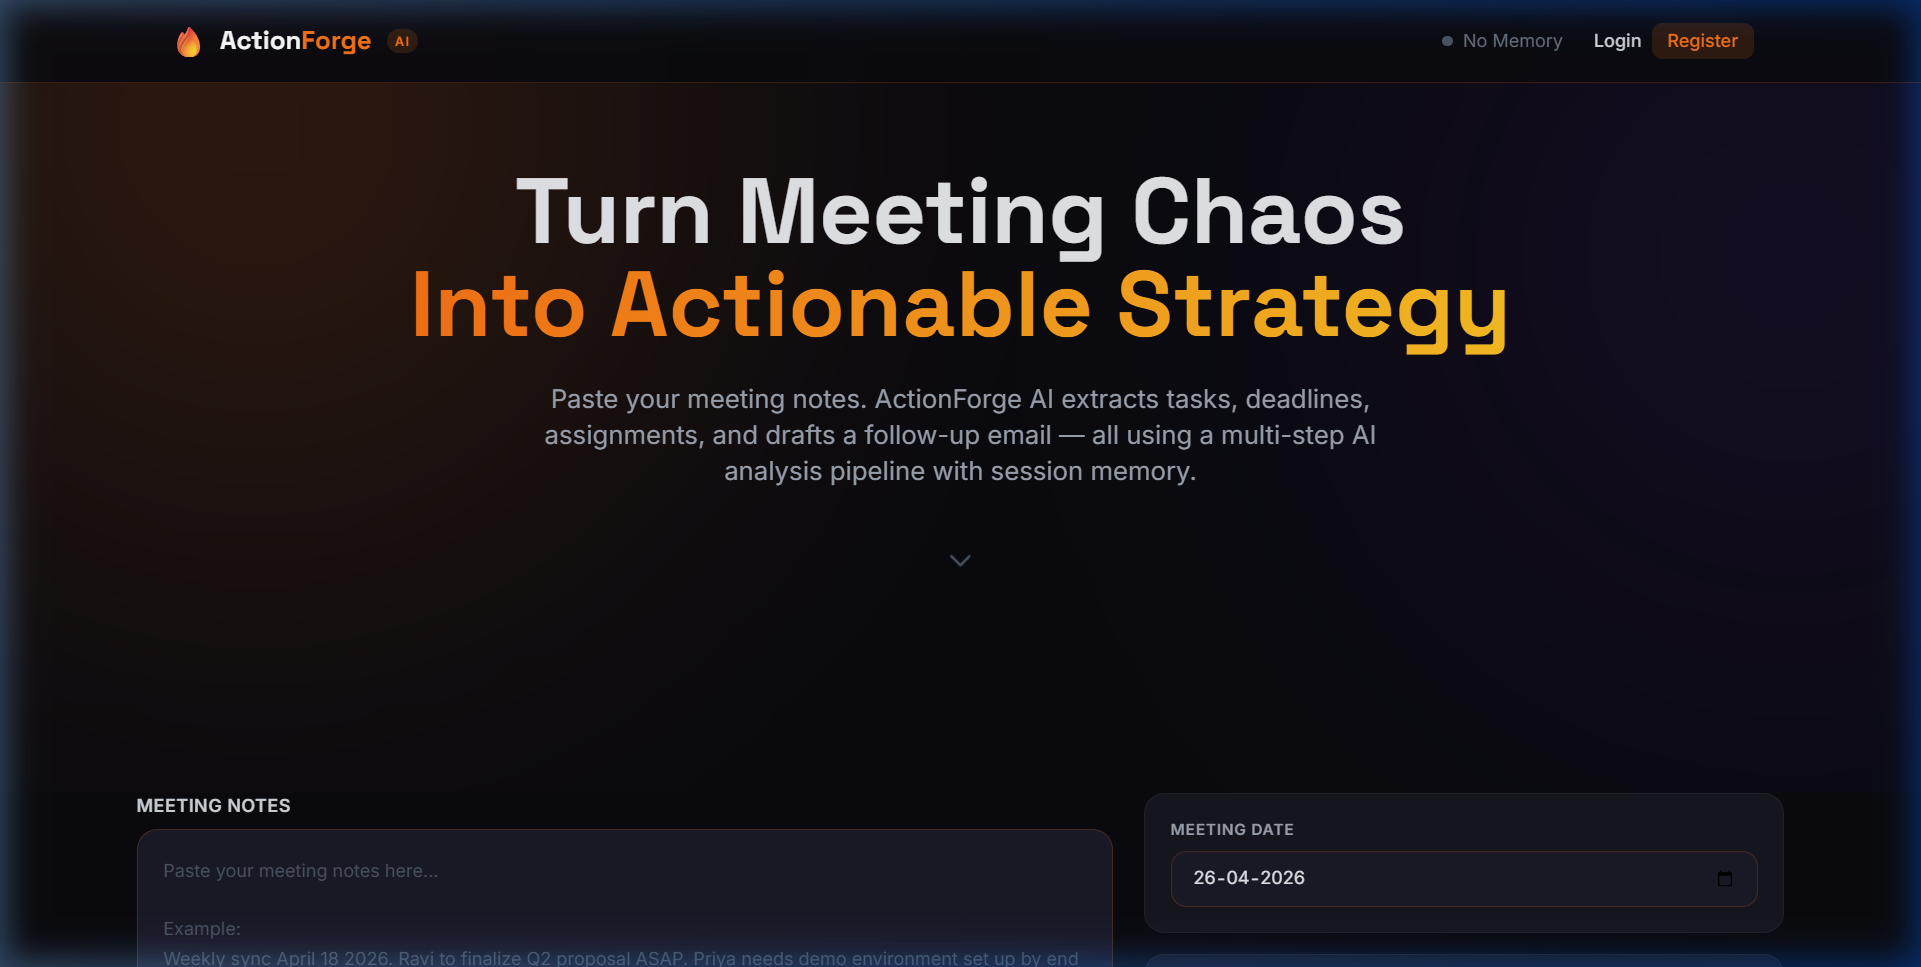
\includegraphics[width=\textwidth]{screenshots/img36_landing_hero.png}
\caption{ActionForge AI Landing Page}
\end{figure}

\textbf{Input Section with Notes \& Controls:}

\begin{figure}[H]
\centering
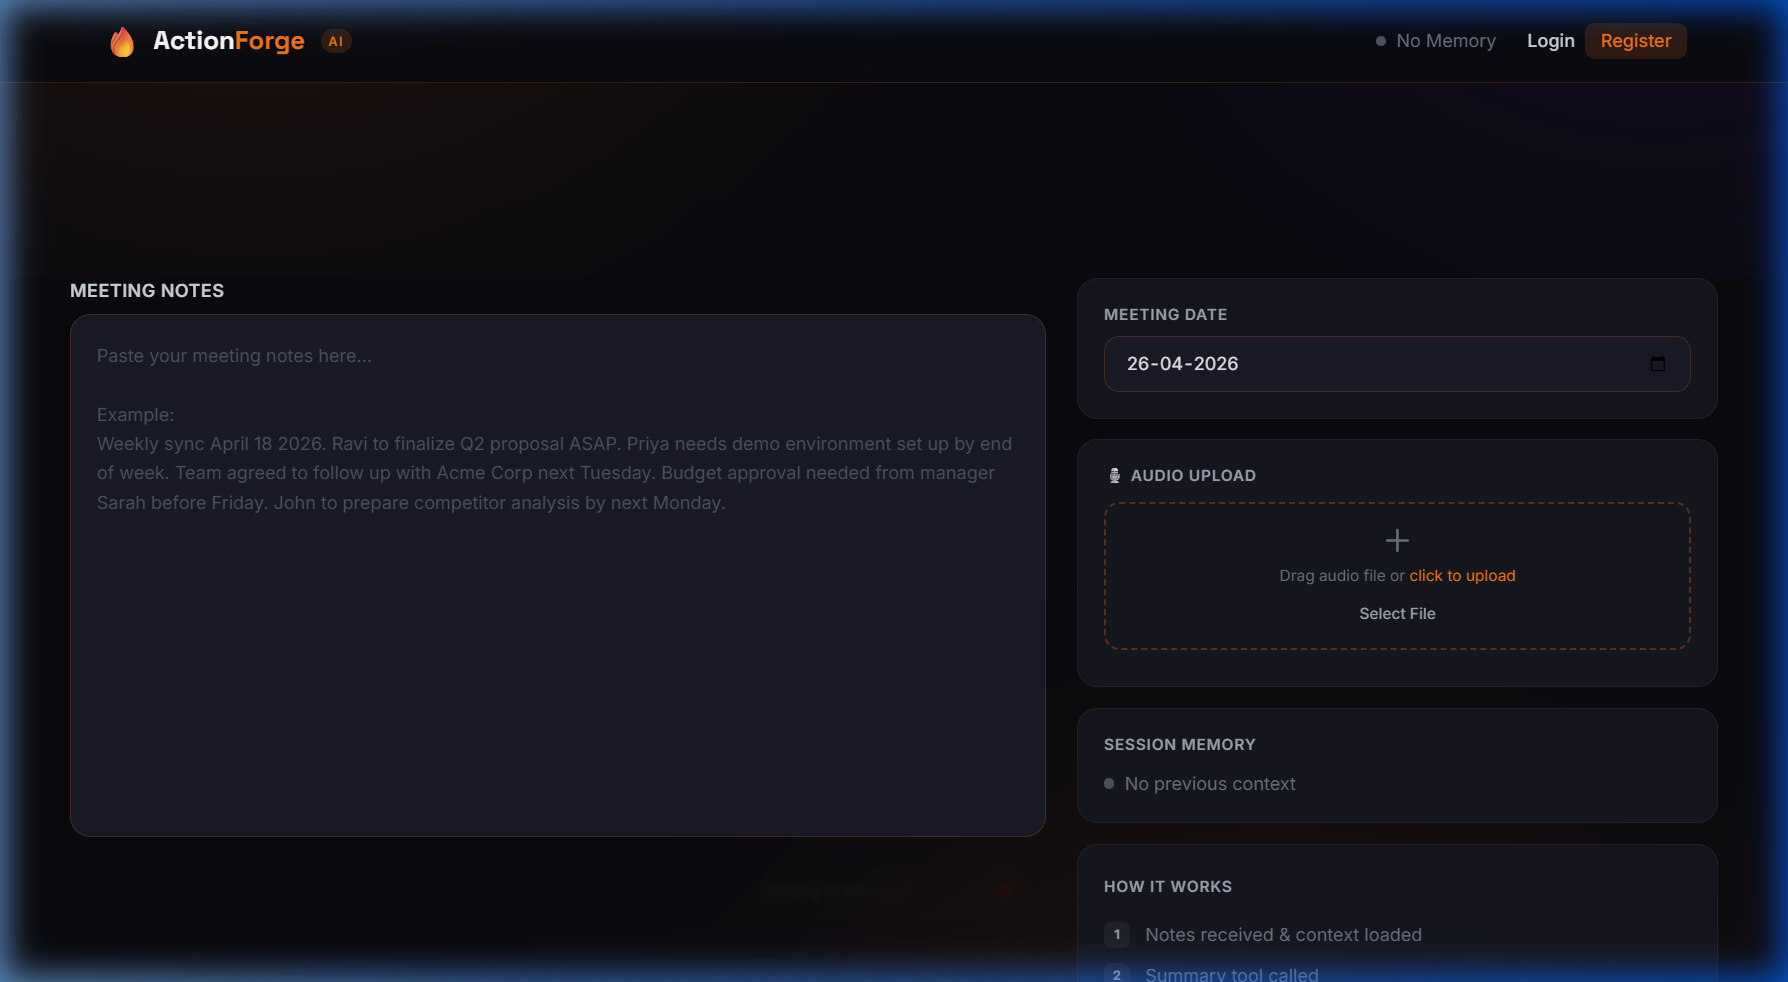
\includegraphics[width=\textwidth]{screenshots/img37_input_section.png}
\caption{Meeting Notes Input Section}
\end{figure}

\textbf{Processing Pipeline Animation:}

\begin{figure}[H]
\centering
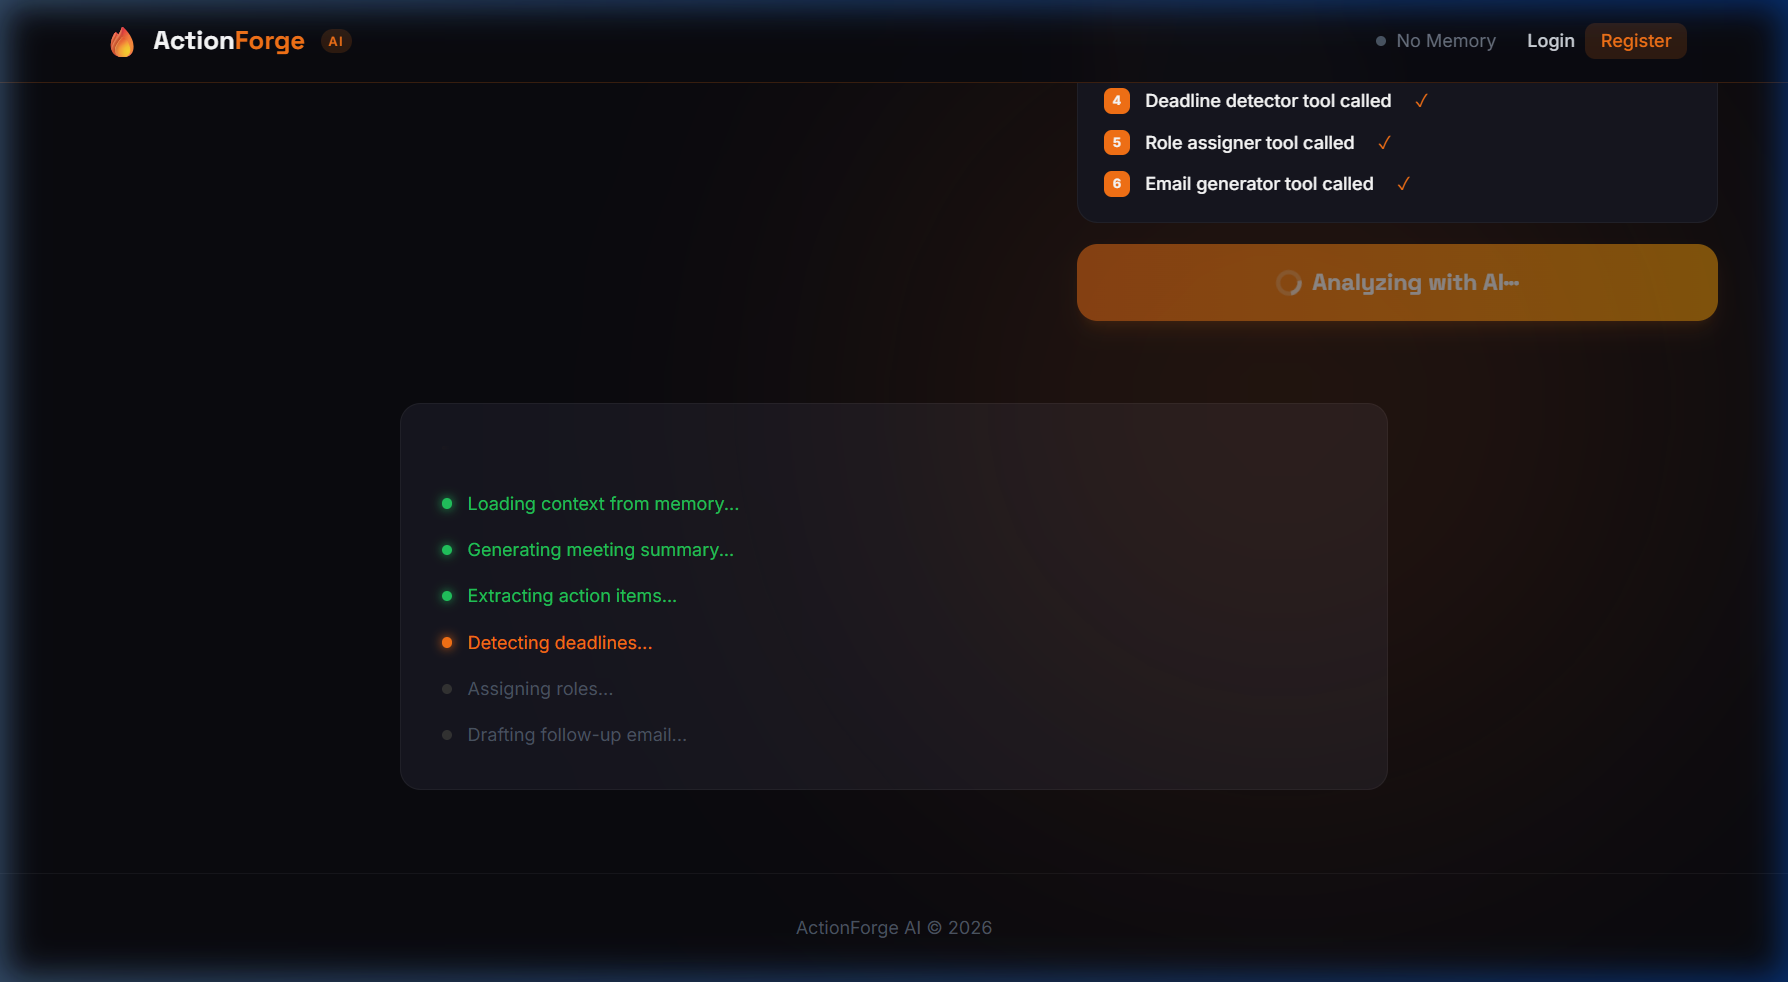
\includegraphics[width=0.8\textwidth]{screenshots/img14_loading_pipeline_png.png}
\caption{Real-time Pipeline Processing Animation}
\end{figure}

\textbf{Executive Summary Result:}

\begin{figure}[H]
\centering
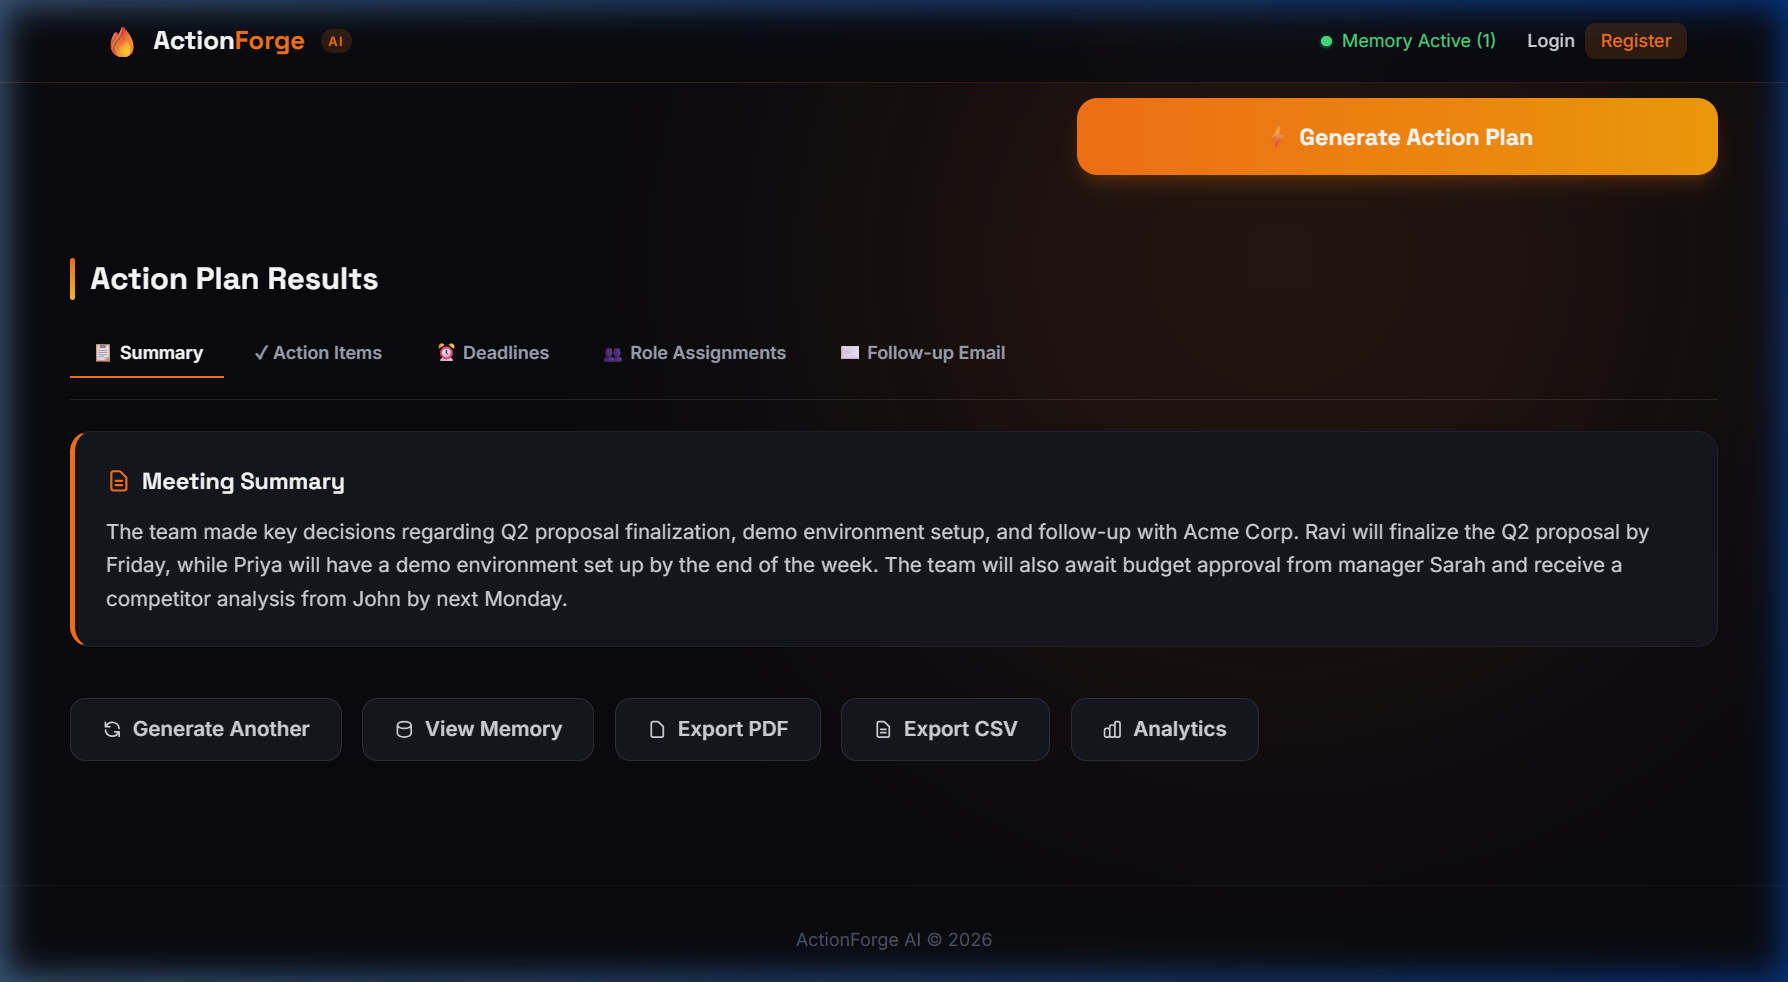
\includegraphics[width=\textwidth]{screenshots/img41_summary_tab_png.png}
\caption{Executive Summary Output generated by AI}
\end{figure}

\textbf{Action Items Table:}

\begin{figure}[H]
\centering
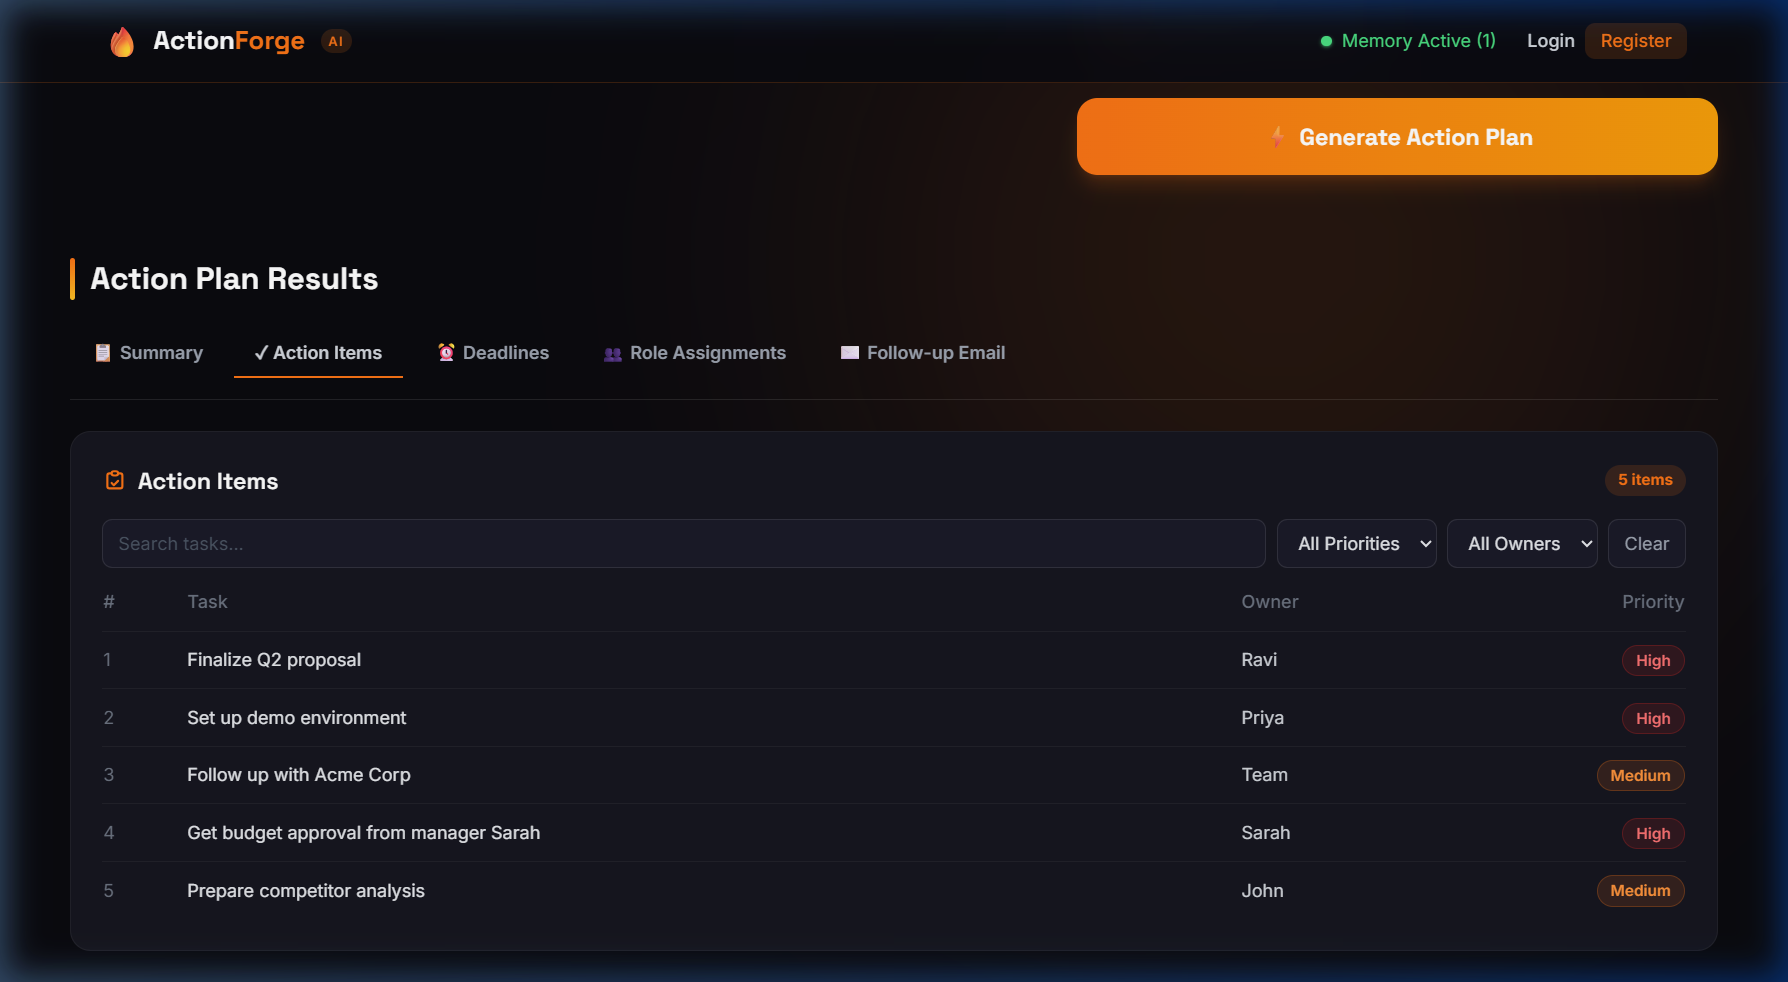
\includegraphics[width=\textwidth]{screenshots/img43_tasks_tab_png.png}
\caption{Extracted Action Items with Assignments and Priorities}
\end{figure}

\textbf{Deadlines with Urgency:}

\begin{figure}[H]
\centering
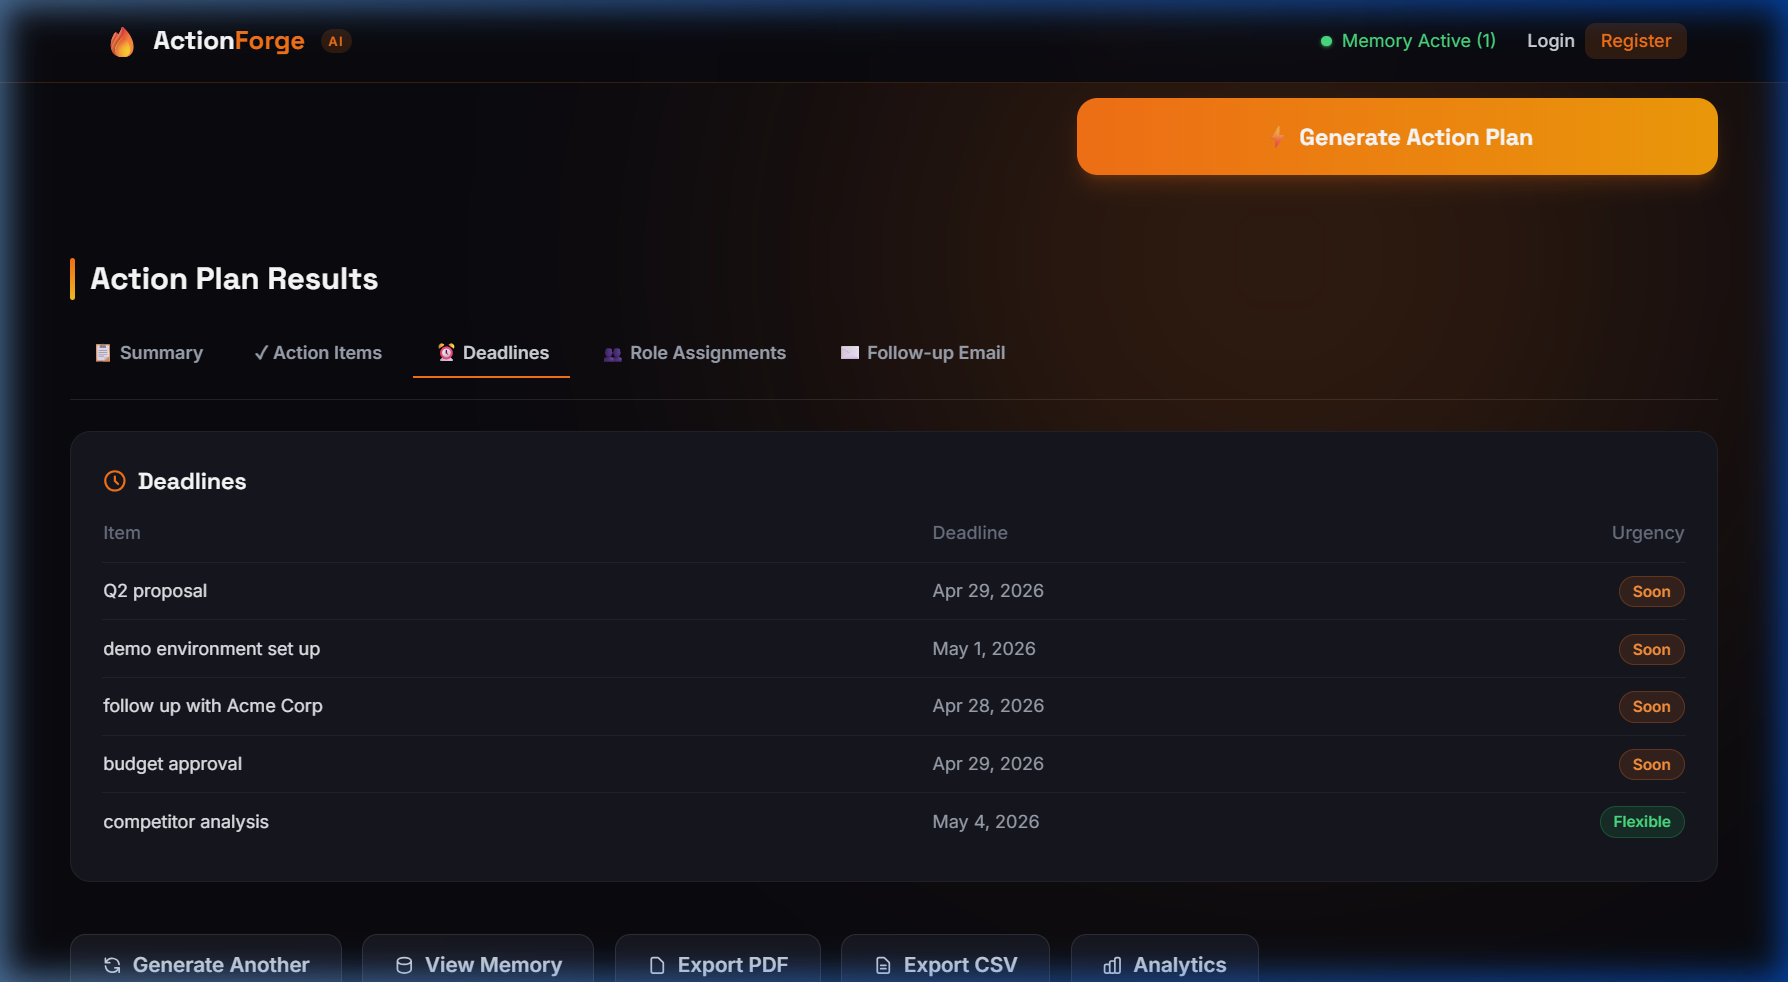
\includegraphics[width=\textwidth]{screenshots/img46_deadlines_tab_png.png}
\caption{Deadlines Tab showing extracted dates and urgency}
\end{figure}

\begin{figure}[H]
\centering
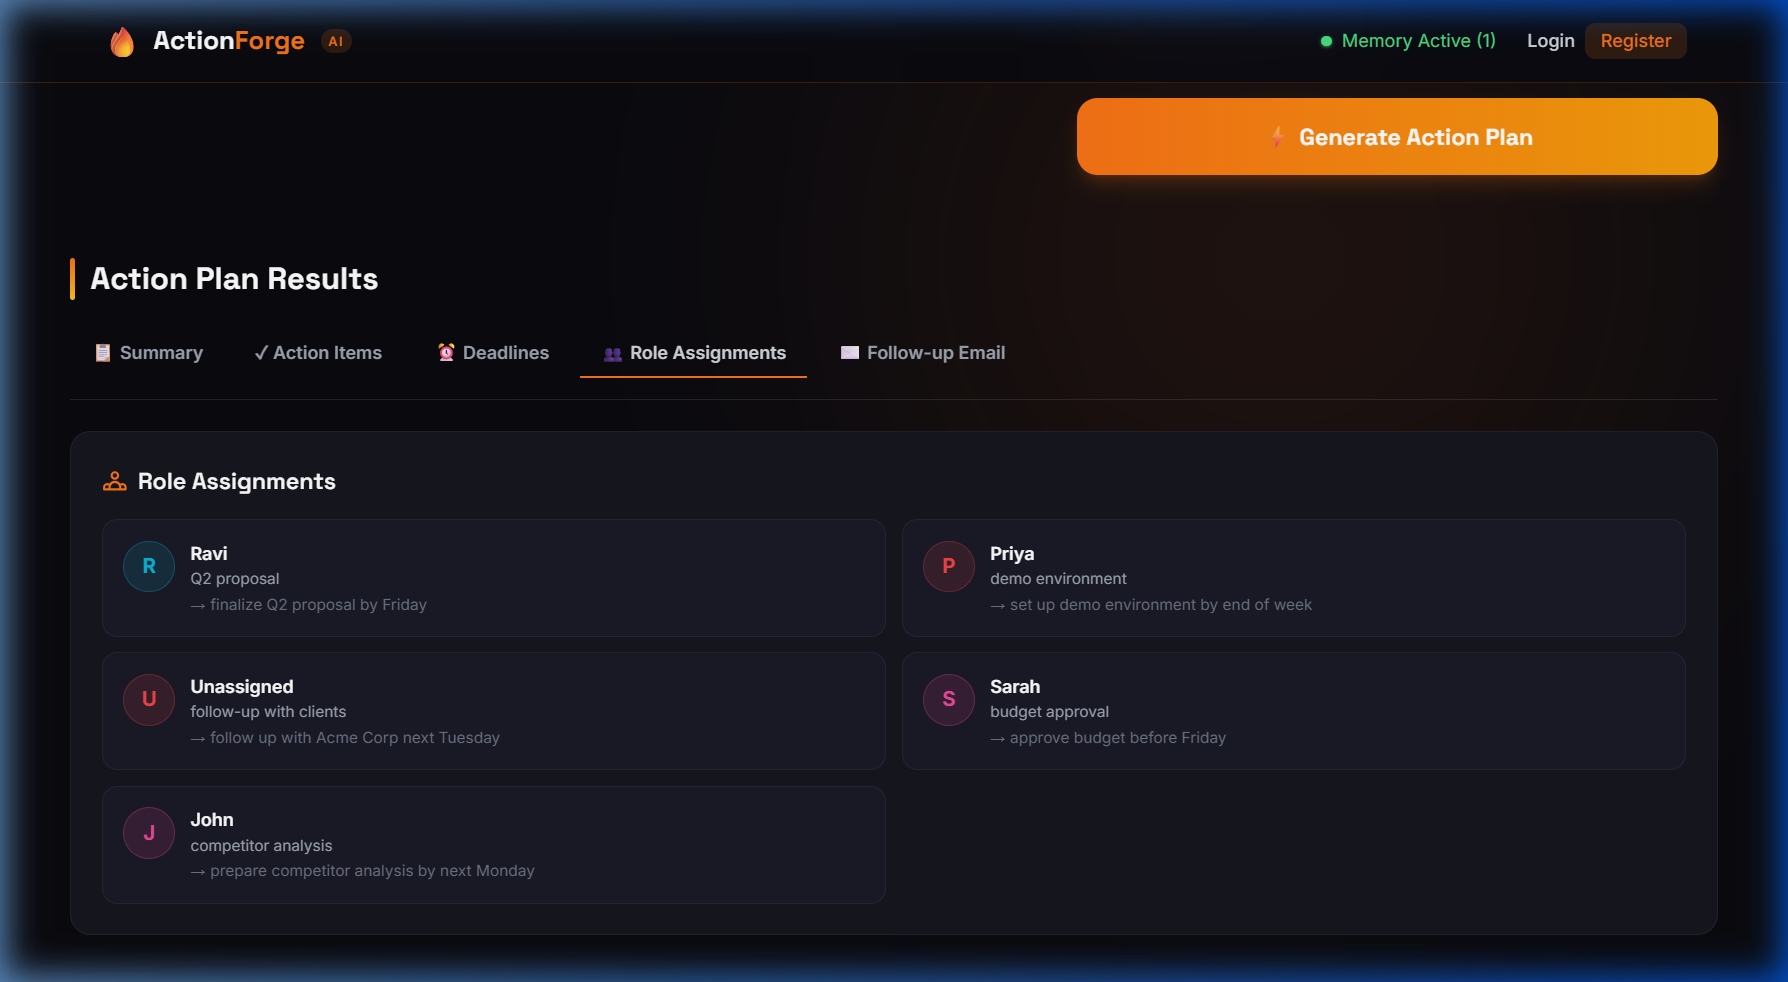
\includegraphics[width=\textwidth]{screenshots/img47_roles_tab_png.png}
\caption{Role Assignments identified from the meeting}
\end{figure}

\textbf{Follow-up Email:}

\begin{figure}[H]
\centering
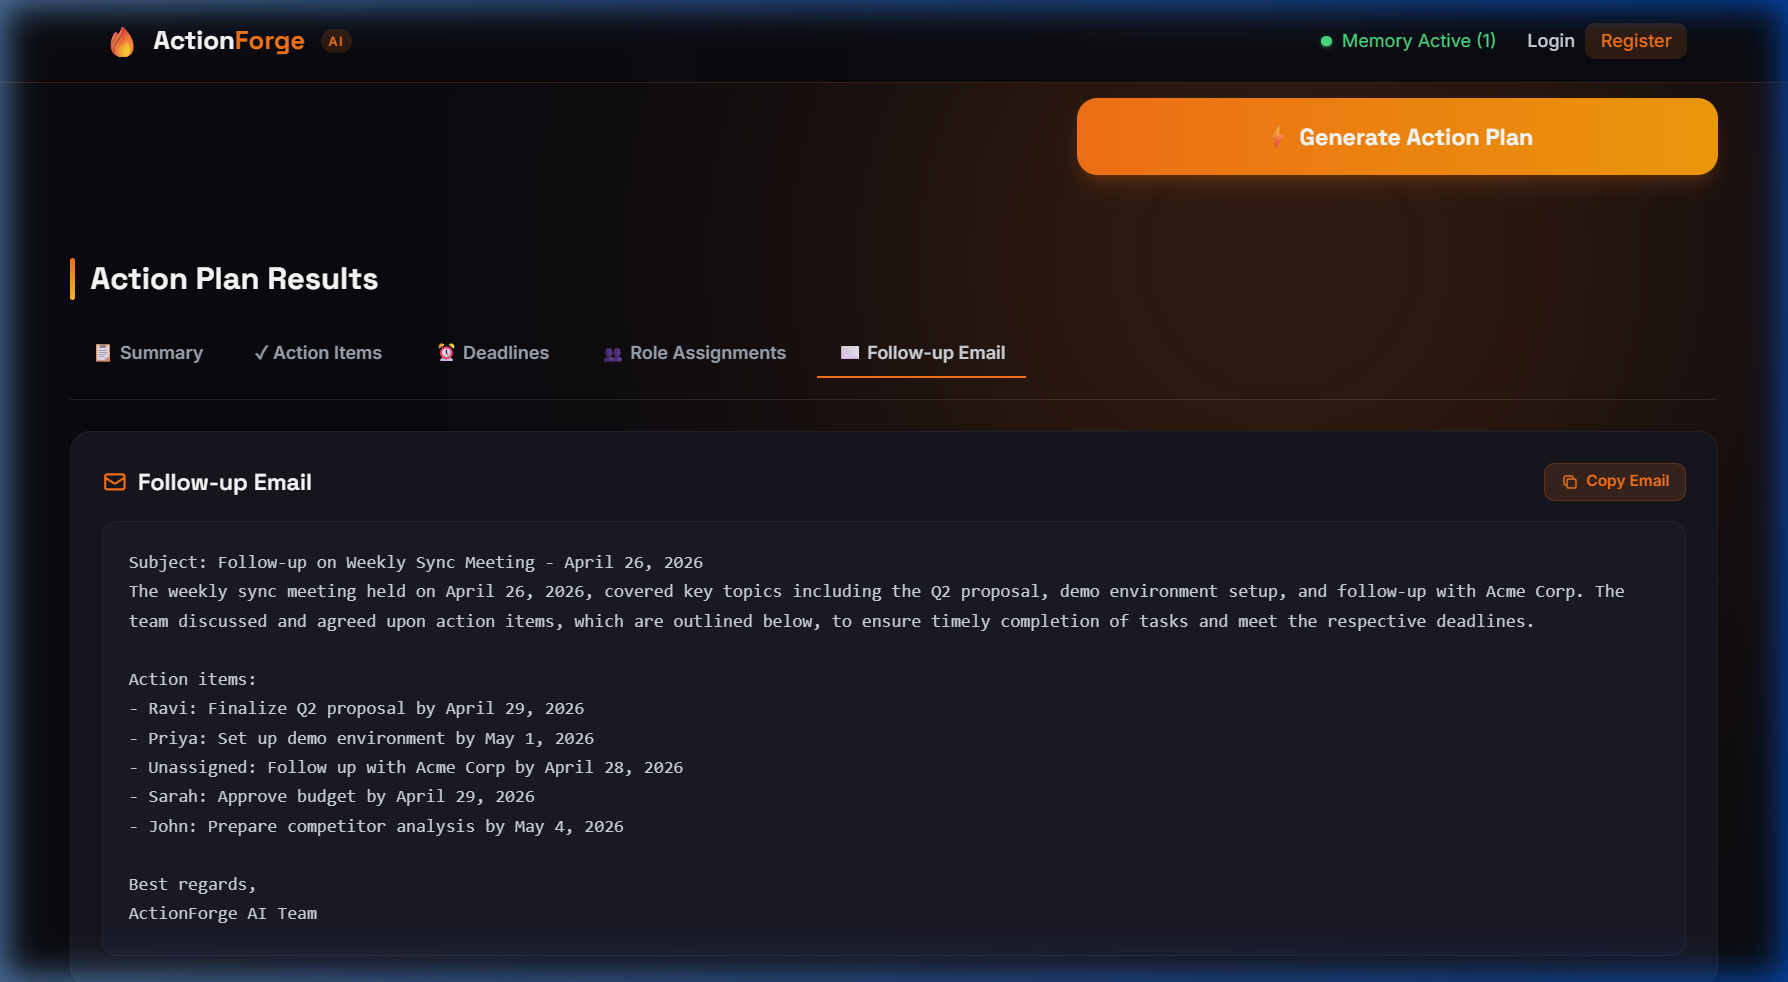
\includegraphics[width=\textwidth]{screenshots/img48_email_tab_png.png}
\caption{AI-Drafted Professional Follow-up Email}
\end{figure}

\textbf{Analytics Dashboard:}

\begin{figure}[H]
\centering
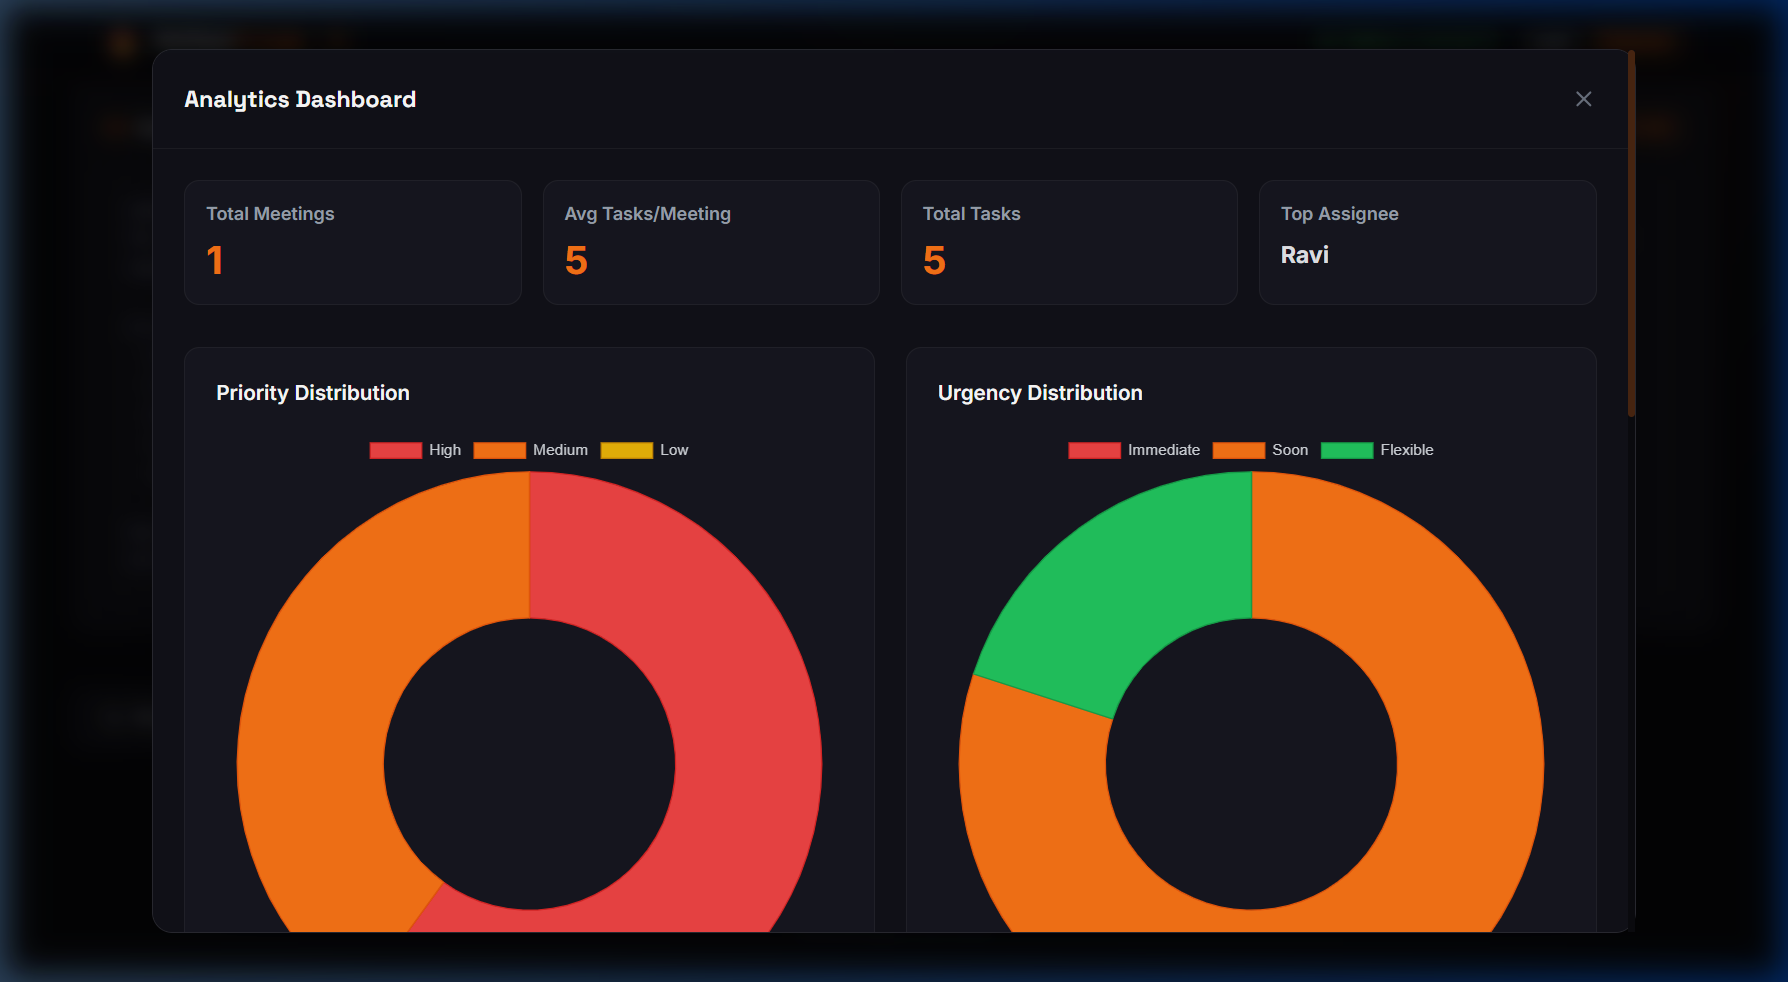
\includegraphics[width=\textwidth]{screenshots/img49_analytics_png.png}
\caption{Analytics Dashboard with visual data distribution}
\end{figure}

\subsection*{Benchmark Results}
The system achieves reliable performance metrics including low response time (5--10 seconds full pipeline), consistent LLM outputs, and accurate task/deadline extraction. The dual-model fallback ensures 99\%+ uptime. Export generation completes within 1--2 seconds. The system performs efficiently under regular usage conditions.


% ══════════════════════════════════════════════════════════════
\section{Advantages \& Limitations}

\subsection{Advantages}

\textbf{AI-Powered Multi-Stage Analysis}
\begin{itemize}
  \item Converts raw meeting notes into five structured outputs in a single request
  \item Uses sequential MCP-style tool pipeline for comprehensive analysis
\end{itemize}

\textbf{Session Memory for Continuity}
\begin{itemize}
  \item Retains context from previous meetings for smarter analysis
  \item Enables cross-meeting tracking of commitments and follow-ups
\end{itemize}

\textbf{Dual-Model Fallback}
\begin{itemize}
  \item Automatically switches to backup LLM if primary fails
  \item Ensures high availability and reliability of AI processing
\end{itemize}

\textbf{Export \& Collaboration}
\begin{itemize}
  \item Professional PDF and CSV exports for documentation
  \item User authentication and session sharing with permission levels
\end{itemize}

\textbf{Real-Time Processing}
\begin{itemize}
  \item Generates complete action plans within seconds
  \item Animated pipeline indicators provide real-time progress feedback
\end{itemize}

\subsection{Limitations}

\textbf{External API Dependency}
\begin{itemize}
  \item Relies on Groq AI services for all text processing
  \item System performance affected by API downtime or rate limits
\end{itemize}

\textbf{In-Memory Storage}
\begin{itemize}
  \item Session memory and user data not persisted to database
  \item Data lost when server restarts
\end{itemize}

\textbf{Limited Historical Data}
\begin{itemize}
  \item No persistent database for long-term meeting history
  \item Analytics limited to current session data
\end{itemize}

\textbf{Basic Authentication}
\begin{itemize}
  \item No JWT tokens or hashed passwords in current implementation
  \item Not production-ready without database-backed auth
\end{itemize}

\textbf{Internet Dependency}
\begin{itemize}
  \item Requires stable internet for LLM API communication
  \item No offline functionality available
\end{itemize}


% ══════════════════════════════════════════════════════════════
\section{Future Enhancements}

\subsection{Scalability Improvements}
\begin{itemize}
  \item Add PostgreSQL/MongoDB for persistent storage of meetings, users, and sessions
  \item Implement caching for repeated queries and LLM responses
  \item Support multi-user environments with high concurrency
  \item Optimize for large-scale deployment with load balancing
\end{itemize}

\subsection{Feature Expansion}
\begin{itemize}
  \item Add task completion tracking and follow-up monitoring
  \item Implement calendar integration (Google Calendar, Outlook)
  \item Provide long-term team performance reports
  \item Enable real-time collaborative editing of action plans
\end{itemize}

\subsection{Cloud Integration}
\begin{itemize}
  \item Deploy backend to cloud platforms (Render, Railway, AWS)
  \item Integrate cloud-based monitoring and logging tools
  \item Enable automated backups and data recovery
  \item Implement CI/CD pipeline for automated deployments
\end{itemize}

\subsection{Mobile Integration}
\begin{itemize}
  \item Develop dedicated mobile applications (Android/iOS)
  \item Push notifications for upcoming deadlines and reminders
  \item Seamless sync between web and mobile platforms
  \item Voice recording directly from mobile app
\end{itemize}

\subsection{Automation}
\begin{itemize}
  \item Auto-generate weekly team summary reports from accumulated meetings
  \item Smart reminders based on upcoming deadlines
  \item Automatic email sending integration (Gmail, Outlook APIs)
  \item Multi-language support for global teams
\end{itemize}


% ══════════════════════════════════════════════════════════════
\section{Conclusion}

ActionForge AI successfully demonstrates how Large Language Models and structured prompt engineering can be combined to transform simple meeting note-taking into an intelligent, automated action planning system. By integrating a multi-stage AI pipeline with session memory, the system provides users with comprehensive outputs --- executive summaries, prioritized task lists, deadline schedules, role assignments, and professional follow-up emails --- all generated from unstructured text input within seconds.

Furthermore, the project highlights the importance of leveraging AI for automated business workflows and proactive team management. Features such as dual-model fallback, analytics dashboards, PDF/CSV exports, and collaboration tools make the system more than just a text processor --- it acts as a virtual meeting assistant that drives accountability and follow-through. Overall, this project showcases a practical implementation of AI in enterprise workflows, with strong potential for future enhancements including database persistence, calendar integration, multi-language support, and mobile applications.


% ══════════════════════════════════════════════════════════════
\section{Appendix}

\subsection{Source Code}
The complete source code is organized into a modular backend (\texttt{backend/}) with separate files for LLM integration, tool pipeline, prompt templates, data models, session memory, export, and collaboration. The frontend is a single-page application (\texttt{frontend/index.html}). The code follows clean architecture principles with clear separation of concerns.

\subsection{Configuration Files}
Configuration files include \texttt{.env} for storing sensitive API keys (Groq, OpenAI) and \texttt{requirements.txt} for Python dependency management. An \texttt{.env.example} file provides a template for new developers setting up the project.

\subsection{API Documentation}
The project provides RESTful API endpoints accessible via FastAPI's auto-generated Swagger UI at \texttt{http://localhost:8000/docs}. Key endpoints include:
\begin{itemize}
  \item \texttt{POST /process\_notes} --- Main pipeline (accepts notes, returns full action plan)
  \item \texttt{GET /memory} --- Retrieve session memory
  \item \texttt{DELETE /memory} --- Clear session memory
  \item \texttt{POST /transcribe\_audio} --- Audio transcription via Whisper
  \item \texttt{POST /export/pdf} --- PDF export
  \item \texttt{POST /export/csv} --- CSV export
  \item \texttt{POST /auth/register} --- User registration
  \item \texttt{POST /auth/login} --- User login
  \item \texttt{POST /sessions/create} --- Create shared session
  \item \texttt{GET /sessions/list} --- List user sessions
  \item \texttt{POST /sessions/\{id\}/share} --- Share session with another user
\end{itemize}

\subsection{GitHub Repository Link}
\url{https://github.com/[your-username]/actionforge-ai}

\end{document}
